\Opensolutionfile{ans}[appendices/vastaukset]

\chapter{Polynomi}
	\section{Käsitteitä}

\qrlinkki{http://opetus.tv/maa/maa2/polynomien-peruskasitteet/}
{Opetus.tv: \emph{polynomien peruskäsitteet} (9:00)}

\qrlinkki{http://opetus.tv/maa/maa2/polynomin-tasmallinen-maaritelma/}
{Opetus.tv: \emph{polynomin täsmällinen määritelmä} (6:10)}

\subsection*{Polynomilausekkeet}

\termi[Polynomit]{polynomi} ovat matematiikassa yleisiä yhden muuttujan laskulausekkeita.
%\termi[Polynomit]{polynomi} ovat matematiikassa ryhmä hyvin yleisiä ja yksinkertaisia yhden muuttujan laskulausekkeita.
%Usein hyödyllinen lauseketyyppi on sellainen joka koostuu muuttujan $x$ ja vakioiden yhteen- ja kertolaskuista.
%Tällaisia lausekkeita kutsutaan muuttujan $x$ \termi[polynomeiksi]{polynomi}.
Esimerkiksi seuraavat lausekkeet ovat muuttujan $x$ polynomeja:
\begin{itemize}
\item $5x^2+x-7$
\item $x^4-6x^3+2x^2-x$
\item $-24x^{100}$
\end{itemize}
Polynomit tunnistaa siitä, että niissä on käytetty muuttujan potenssien lisäksi vain yhteen-, vähennys- ja kertolaskuja. Esimerkiksi seuraavat muuttujan $x$ lausekkeet \emph{eivät ole} polynomeja:
\begin{itemize}
\item $2/x$
\item $\sqrt{x}+2$
\end{itemize}
Yleisin muuttujakirjain on $x$, mutta myös muita kirjaimia voidaan käyttää
merkitsemään muuttujia. Esimerkiksi $2y^5+y^4-1$ on muuttujan $y$ polynomi ja
$-A^3+2A^2-1$ on muuttujan $A$ polynomi.

Polynomilausekkeet ovat summia, joiden yhteenlaskettavia kutsutaan \termi[termeiksi]{termi}. (Termit, joita edeltää miinusmerkki, voidaan käsittää negatiivisten lukujen yhteenlaskuina.)

Esimerkiksi polynomin $5x^2+x-7$ termit ovat $5x^2$, $x$ ja $-7$. Kukin termi on muuttujan potenssi kerrottuna jollakin vakiolla, joka voi olla myös negatiivinen. Termi voi olla myös \termi[vakiotermi]{vakiotermi}, joka ei sisällä muuttujaa. Esimerkiksi $-7$ on vakiotermi.

Yhden termin polynomeista käytetään erityisnimitystä \termi[monomi]{monomi} ja kahden termin polynomi on puolestaan \termi[binomi]{binomi}.

Termin muuttujan eksponenttia kutsutaan termin \termi[asteeksi]{termi!aste}.
Vakiotermin aste on nolla.
%Erikoistapaus termistä on nollannen asteen termi, joka on vain vakio eli \termi{vakiotermi}.
Polynomin \termi[aste]{polynomi!aste} (käytetään myös nimitystä \termi[asteluku]{polynomi!asteluku}) on suurin sen termien asteista.

Koska polynomilauseke koostuu potenssien summista ja yhteenlasku on vaihdannainen, termien paikkaa polynomissa voidaan vapaasti vaihtaa. Siksi esimerkiksi polynomi $\frac{1}{3}y^3+y^2-3$ voidaan kirjoittaa myös järjestyksessä $y^2-3+\frac{1}{3}y^3$. Yleensä polynomien termit kirjoitetaan niiden asteen perusteella laskevaan järjestykseen niin, että korkeimman asteen termi kirjoitetaan ensin.

\begin{esimerkki}
Polynomilausekkeen $x^4-2x^3+5$ termit ovat $x^4$, $-2x^3$ ja $5$.
Ensimmäinen termi $x^4$ on neljännen asteen termi. Termin $-2x^3$ aste on kolme, ja vakiotermin $5$ aste on nolla.
Koko polynomin aste on neljä, koska se on termien asteista suurin.
\end{esimerkki}

%Huomaa, että polynomilauseke pitää sieventää ennen asteen määrittämistä.
%Määritetään vaikkapa polynomin $x^5-4x^2+6x^3+3-x^5-x$ aste.
%Summataan ensin termejä niin, että
%polynomissa on vain yksi termi jokaista astetta:
%\[x^5-4x^2+6x^3+3-x^5-x = 6x^3-4x^2-x+3.\]
%Nyt nähdään, että polynomin aste on 3.

%\laatikko{
%Polynomi $P$, joka on astetta $n$, voidaan aina sieventää muotoon
%\[P(x) = a_n x^n + a_{n-1} x^{n-1} + \ldots + a_1 x + a_0,\]
%missä $a_0, a_1, \ldots, a_n$ ovat vakioita ja $a_n \neq 0$.
%}

\subsection*{Polynomifunktion arvo}

\qrlinkki{http://opetus.tv/maa/maa2/polynomiesimerkkeja/}
{Opetus.tv: \emph{polynomiesimerkkejä} (7:43 ja 6:59)}

Polynomi määrittää funktion, jota kutsutaan \termi[polynomifunktioksi]{polynomifunktio}. Esimerkiksi polynomi $2x^2+2x-1$ määrittää funktion $P(x)=2x^2+2x-1$. Tämän funktion arvoja voidaan laskea sijoittamalla lukuja muuttujan $x$ paikalle:
\begin{align*}
P(2) & = 5\cdot 2^2-3\cdot 2+2 = 20 - 6 + 2 = 16 \\
P(-1) & = 5(-1)^2-3(-1)+2 = 5 + 3 + 2 = 10 \\
P(-3) & = 5(-3)^2-3(-3)+2 = 45 + 9 + 2 = 56.
\end{align*}

Toisinaan polynomeja ja polynomifunktioita käsitellään kuin ne olisivat sama asia.
Voidaan esimerkiksi sanoa ''polynomi $P(x)=2x+1$'', vaikka yleensä $P(x)$-merkintää käytetään funktioista.

%Samalla polynomifunktiolla voi olla useampia esityksiä polynomilausekkeena.
%Esimerkiksi jos $P(x) = x^2-x^2+x+1$ ja $Q(x) = x+1$, $P$ ja $Q$ ovat samat
%funktiot koska $x^2 - x^2 = 0$ kaikilla reaaliluvuilla x. Siis saman
%polynomifunktion eri esityksissä lausekkeina suurimman termin aste voi olla
%eri, esimerkiksi $P$:ssä se on 2 ja $Q$:ssa 1. Useimmiten kiinnostavin on
%kuitenkin pienin mahdollinen aste, jolloin polynomifunktion $P$ aste olisi
%myös 1.

\subsection*{Polynomien yhteen- ja vähennyslasku}

\qrlinkki{http://opetus.tv/maa/maa2/polynomien-yhteen-ja-vahennyslasku/}
{Opetus.tv: \emph{polynomien yhteen- ja vähennyslasku} (7:36)}

Polynomeja voidaan laskea yhteen summaamalla samanasteiset termit. Tätä varten on kätevää ensin ryhmitellä polynomin samanasteiset termit vierekkäin.

\begin{esimerkki}
Laske polynomien $5x^2-x+5$ ja $3x^2-1$ summa.
   \begin{align*}
        (\textcolor{blue}{5x^2} \textcolor{red}{{}-x} + 5) + (\textcolor{blue}{+3x^2} -1) 
        &=\textcolor{blue}{5x^2} \textcolor{red}{{}-x} + 5  \textcolor{blue}{{}+3x^2} -1 \\
        &=\textcolor{blue}{5x^2+3x^2} \textcolor{red}{{}-x} +5-1\\
        &=\textcolor{blue}{(5+3)x^2} \textcolor{red}{{}-x}+(5-1)\\
        &=\textcolor{blue}{8x^2} \textcolor{red}{{}-x}+4.
    \end{align*}
\end{esimerkki}

Samalla tavalla polynomeja voidaan vähentää toisistaan.

\begin{esimerkki}
    Laske polynomien $14x^3+69$ ja $3x^3+2x^2+x$ erotus.
    \begin{align*}
        (\textcolor{green}{14x^3} + 69) - (\textcolor{green}{3x^3} \textcolor{blue}{{}+ 2x^2} \textcolor{red}{{}+x})
        &= \textcolor{green}{14x^3} + 69 \textcolor{green}{{}-3x^3} - 
            \textcolor{blue}{2x^2} \textcolor{red}{{}-x} \\
        &= \textcolor{green}{14x^3{}-3x^3} \textcolor{blue}{{}-2x^2} \textcolor{red}{{}-x} + 69 \\
        &= \textcolor{green}{(14{}-3)x^3} \textcolor{blue}{{}-2x^2} \textcolor{red}{{}-x} + 69 \\
        &= \textcolor{green}{11x^3} \textcolor{blue}{{}-2x^2} \textcolor{red}{{}-x} + 69
    \end{align*}
\end{esimerkki}
    
Samanasteisten termien yhteen- ja vähennyslasku perustuu siihen, että reaalilukujen osittelulain (ks. Vapaa matikka 1) nojalla vakiokerroin voidaan
ottaa yhteiseksi tekijäksi:
\[
ax^n+bx^n=(a+b)x^n.
\]

  
\begin{esimerkki}
Olkoon polynomit $P(x)=x+1$ ja $Q(x)=3x^2-2x+5$. Määritä summa $P(x)+Q(x)$.
   \begin{align*}
        P(x)+Q(x)&=(x+1)+(3x^2-2x+5) = x+1+3x^2-2x+5 \\
                 &= 3x^2+x-2x+1+5 =3x^2-x+6.
    \end{align*}
\end{esimerkki}

Kun laskurutiinia eli varmuutta on tarpeeksi, voi yllä olevasta esimerkistä jättää yksi tai kaksi välivaihetta pois.

% \begin{esimerkki}
% Määritä polynomien $R(x)=-4x^4+3x^3-x$ ja $S(x)=-3x^3+5x^2+2x$ summa.
%    \begin{align*}
%         R(x)+S(x)=(-4x^4+3x^3-x)+(-3x^3+5x^2+2x) =-4x^4+5x^2+x.
%     \end{align*}
% \end{esimerkki}

\begin{esimerkki}
    Laske polynomien $P(x)$ ja $R(x)$ erotus, kun $P(x)=x+1$ ja $R(x)=-4x^4+3x^3-x$.
   \begin{align*}
        P(x)-R(x) & =(x+1)-(-4x^4+3x^3-x) =x+1+4x^4-3x^3+x \\
        & =4x^4-3x^3+x+x+1 = 4x^4-3x^3+2x+1.
    \end{align*}
\end{esimerkki}

Yhteenlasketut ja vähennetyt polynomit sievennetään yleensä perusmuotoon, jossa on vain yksi termi kutakin astetta kohti. Tämä tehdään esimerkiksi silloin, kun selvitetään polynomin aste.

\begin{esimerkki} Mikä on polynomin $P(x)=(x^2+2x+1)-(x^2+2)$ aste?

\[
P(x)=x^2+2x+1-x^2-2=2x-1.
\]
Ensisilmäyksellä polynomin asteen voisi ajatella olevan 2, mutta tässä tapauksessa toisen asteen termit häviävät sievennettäessä ja asteluku onkin 1.
\end{esimerkki}


\Harjoitustehtavat

\paragraph*{Opi perusteet}

\begin{tehtava}
    Täydennä taulukko.
        
    \begin{tabular}{|c|c|c|c|c|}
                                                                                           \hline
             & termien   & korkeimman asteen & polynomin &            \\
polynomi     & lukumäärä & termin kerroin    & asteluku  & vakiotermi \\ \hline
$-2x^2+6x$   &        2  &         $-2$      &       2   &    0       \\ \hline 
$7x^3-x-15$  &           &                   &           &            \\ \hline 
             &        2  &          $-9$     &       2   &    5       \\ \hline 
             &        3  &          $-1$     &       5   &    $-17$   \\ \hline 
             &        4  &                   &       3   &            \\ \hline 
             &        1  &          -5       &       99  &            \\ \hline                           
    \end{tabular}
    \begin{vastaus}
    Värilliset kohdat voivat olla jotain muutakin.
    
    \begin{tabular}{|c|c|c|c|c|}
                                                                                           \hline
             &                   & korkeimman asteen &                     &            \\
polynomi     & termien lukumäärä & termin kerroin    & polynomin asteluku  & vakiotermi \\ \hline
$-2x^2+6x$   &        2          &         $-2$      &       2             &    0       \\ \hline 
$7x^3-x-15$  &        3          &           7       &       3             &    $-15$   \\ \hline 
$-9x^2+5$    &        2          &          $-9$     &       2             &    5       \\ \hline 
$-x^5\textcolor{blue}{+4x}-17$%
             &        3          &          $-1$     &       5             &    $-17$   \\ \hline 
$\textcolor{blue}{8}x^3\textcolor{blue}{-x^2+4x}-17$%
             &        4          &\textcolor{blue}{8}  &       3             &\textcolor{blue}{7}\\ \hline 
$-5x^{99}$   &        1          &          $-5$     &       99            &         0      \\ \hline                           
     \end{tabular}
     \end{vastaus}
\end{tehtava}



\begin{tehtava}
    Mitkä seuraavista ovat polynomeja?
    \begin{enumerate}[a)]
        \item $\frac{1}{x}$
       %\item $x^3+4x$
        \item $5x-125$
       %\item $2^x$
        \item $\sqrt{x}+1$
        \item $3x^4+6x^2+9$
        \item $\sqrt{2}x-x$
        \item $4^x+5x+6$
    \end{enumerate}
    \begin{vastaus}
        \begin{enumerate}[a)]
            \item Ei ole.
           %\item On.
            \item On.
           %\item Ei ole.
            \item Ei ole.
            \item On.
            \item On.
            \item Ei ole.
        \end{enumerate}
    \end{vastaus}
\end{tehtava}

\begin{tehtava}
    Olkoot $P(x)=x^2+5$ ja $Q(x)=x^3-1$. Laske
    \begin{enumerate}[a)]
        \item $P(2)$
        \item $Q(1)$
        \item $P(-7)$
        \item $Q(-4)$.
    \end{enumerate}
    \begin{vastaus}
        \begin{enumerate}[a)]
            \item $9$ % 2^2 + 5 = 4 + 5 
            \item $0$ % 1^3 - 1
            \item $54$ % (-7)^2 + 5 = 49 + 5 
            \item $-65$ % (-4)^3 - 1 = -64 -1
        \end{enumerate}
    \end{vastaus}
\end{tehtava}

%\begin{tehtava}
%    Olkoot $P(x)=x^2+3x+4$ ja $Q(x)=x^3-10x+1$. Laske:
%    \begin{enumerate}[a)]
%        \item $P(-1)$
%        \item $Q(-2)$
%        \item $P(3)$
%        \item $Q(0)$
%    \end{enumerate}
%    \begin{vastaus}
%        \begin{enumerate}[a)]
%            \item $2$
%            \item $13$
%            \item $22$
%            \item $1$
%        \end{enumerate}
%    \end{vastaus}
%\end{tehtava}

\begin{tehtava}
    Olkoot $P(x)=x^2+3x+4$ ja $Q(x)=x^3-10x+1$. Sievennä
    \begin{enumerate}[a)]
        \item $P(x)+Q(x)$
        \item $P(x)-Q(x)$
        \item $Q(x)-P(x)$
        \item $2P(3)+Q(2)$.
    \end{enumerate}
    \begin{vastaus}
        \begin{enumerate}[a)]
            \item $x^3+x^2-7x+5$ % x^2+3x+4 + x^3-10x+1
            \item $-x^3+x^2+13x+3$ % x^2+3x+4 -(x^3-10x+1) = x^2+3x+4 -x^3+10x-1
            \item $x^3-x^2-13x-3$ % 
            \item $33$ % 2*(3^2+3*3+4) +  2^3-10*2+1 = 2*(9+9+4)+8-20+1 =44-11 =33
        \end{enumerate}
    \end{vastaus}
\end{tehtava}

%\begin{tehtava}
%	Mikä on/mitkä ovat polynomin $P(x) = x^5-3x^3+2x-1$
%	\begin{enumerate}[a)]
%		\item aste
%		\item termit
%		\item kolmannen asteen termi
%		\item vakiotermi
%	\end{enumerate}
%
%	\begin{vastaus}
%		\begin{enumerate}[a)]
%			\item $5$
%			\item $x^5$, $-3x^3$, $2x$, $-1$
%			\item $-3x^3$
%			\item $-1$
%		\end{enumerate}
%	\end{vastaus}
%\end{tehtava}

%\begin{tehtava}
%	Mitkä on seuraavien polynomien asteet?
%	\begin{enumerate}[a)]
%		\item $x^2 + 3x - 5$
%		\item $100 + x$
%		\item $3x^3 + 90x^8 + 2x$
%		\item $12x^1 + 34x^2 + 56x^3 + 78x^5 + 90x^5$
%	\end{enumerate}
%
%	\begin{vastaus}
%		\begin{enumerate}[a)]
%			\item $2$
%			\item $1$
%			\item $8$
%			\item $5$
%		\end{enumerate}
%	\end{vastaus}
%\end{tehtava}

% \begin{tehtava}
%     Sievennä
%     \begin{enumerate}
%         \item $(2x + 3) + x $
%         \item $(3x - 1) + (-x + 1)$
%         \item $(5x + 10) + (6x - 6) - (x + 3)$
%     \end{enumerate}
%     \begin{vastaus}
%         \begin{enumerate}
%             \item $3x + 3$
%             \item $2x$
%             \item $10x - 1$
%         \end{enumerate}
%     \end{vastaus}
% \end{tehtava}

\paragraph*{Hallitse kokonaisuus}

\begin{tehtava}
    Sievennä
    \begin{enumerate}
        \item $(x^2 - 2x + 1) + (-x^2 + x) $
        \item $(3y^3 + 2y^2  + y) - (-y^2 + y)$
        \item $(z^{10} - z^6 + z^2 + 1) + (z^{10} + 2z^8 - 3z^6) - (z^4 - 3)$.
    \end{enumerate}
    \begin{vastaus}
        \begin{enumerate}
            \item $-x + 1$
            \item $3y^3 + 3y^2$
            \item $2z^{10} + 2z^8 - 4z^6 - z^4 + z^2 + 4$
        \end{enumerate}
    \end{vastaus}
\end{tehtava}

\begin{tehtava}
	Mitkä ovat seuraavien polynomifunktioiden asteet, ts. sievennettyjen muotojen asteet?
	\begin{enumerate}[a)]
		\item $x+5-x$
		\item $x^2+x-2x^2$
		\item $4x^5+x^2-4-x^2$
		\item $x^3+2x^5-x-3x^5+3x^2+5+x^5$
		\item $x^4-2x^3+x-1+x^3-x^4+x^3$
	\end{enumerate}

	\begin{vastaus}
		\begin{enumerate}[a)]
			\item $0$
			\item $2$
			\item $5$
			\item $3$
			\item $1$
		\end{enumerate}
	\end{vastaus}
\end{tehtava}

% Hämäävä tehtävä
% \begin{tehtava}
% 	Sievennä.
% 	\begin{enumerate}[a)]
% 		\item $2 + x$
% 		\item $3x - 1 + 2x^2$
% 		\item $x^3 - \dfrac{2}{3}x^5 + 2x^4 $
% 		\item $1 - 15x + \pi x^{10} + 2$
% 		\item $-2x + 3 + 5x - 5x^2 - 5$
% 	\end{enumerate}
%
% 	\begin{vastaus}
% 		\begin{enumerate}[a)]
% 			\item $x + 2$
% 			\item $2x^2 + 3x - 1$
% 			\item $-\dfrac{2}{3}x^5 + 2x^4 + x^3 $
% 			\item $\pi x^10 - 15x + 3$
% 			\item $-5x^2 + 3x - 2$
% 		\end{enumerate}
% 	\end{vastaus}
% \end{tehtava}

\begin{tehtava}
	Mitkä seuraavista polynomilausekkeista esittävät samaa polynomifunktiota kuin
	$x^3+2x+1$?
	\begin{enumerate}[a)]
		\item $2x+x^3+1$
		\item $x^2+2x+1$
		\item $x+2x^3+1 - (x^3+x)$
		\item $15+x^4+2x+x^3-x^4-14$
	\end{enumerate}
	\begin{vastaus}
		a) ja d)
	\end{vastaus}
\end{tehtava}

\begin{tehtava}
	Sievennä polynomifunktiot ja laske funktioiden arvot muuttujan arvoilla $1$, $-1$ ja $3$.
	\begin{enumerate}[a)]
		\item $P(x)=(x^3-4x+5)+(-x^3+x^2+4x-2)$
		\item $Q(x)=(2x^3+x^2-10x)-(3x^3-4x^2+5x)$
		\item $R(x)=4(2x-4)+(-x^3+1)$
		\item $S(x)=-(2x^2-x+8)+6(x^5-3x^2+1)-2(3x^5-10x^2)$
	\end{enumerate}
	
	\begin{vastaus}
		\begin{enumerate}[a)]
			\item $P(x)=x^2+3$, $P(1)=-2$, $P(-1)=-2$ ja $P(3)=5$
			\item $Q(x)=-x^3+5x^2-15x$, $Q(1)=-11$, $Q(-1)=-9$ ja $R(3)=-27$
			\item $R(x)=-x^3+8x-15$, $R(1)=-8$, $R(-1)=-6$ ja $R(3)=-18$
			\item $S(x)=-2$, $S(1)=-2$, $S(-1)=-2$ ja $S(3)=-2$
		\end{enumerate}

	\end{vastaus}


\end{tehtava}

	%polynomin käsite, eli lähinnä terminologiaa: lauseke, termi, monomi, binomi, polynomi, polynomin aste, vakiotermi
	%funktiomerkintä P(x), polynomin arvo
	%samannimisten termien yhdistäminen, sulkujen kanssa pelaaminen tyyliin x-(x-1)=x-x+1=1
	\chapter{Polynomien kertolasku}

\subsection*{Polynomin kertominen monomilla}

Polynomeja voi kertoa keskenään aivan kuten reaalilukuja. Yksinkertaisin tapaus on polynomin kertominen monomilla.

\subsubsection*{Esimerkkejä}
\begin{itemize}
    \item $2x(3x^2+5x+7) = 6x^3+10x^2+14x$
    \item $5x(3y^2+4y) = 15xy^2+20xy$
    \item $x(y+z) = xy+xz$
\end{itemize}

\subsection*{Kahden binomin tulo}

Toinen yksinkertainen tapaus on kahden binomin tulo. Tällöin kerrotaan termeittäin ja summataan.

\subsubsection*{Esimerkkejä}
\begin{itemize}
    \item $(x+y)(z+w) = xz+xw+yz+yw$
    \item $(ax+by)(x+y) = ax^2+axy+bxy+by^2 = ax^2+(a+b)xy+by^2$
    \item $(x-5)(x-7) = x^2-7x-5x+35 = x^2-12x+35$
\end{itemize}

\subsection*{Yleinen kertolasku}

Osittelulain nojalla kahden polynomin tulo saadaan laskemalla yhteen kaikki
termit, jotka saadaan kertomalla termi ensimmäisestä ja toinen termi toisesta
polynomista.

\newcommand{\pbezier}[4]{
	\pgfmathsetmacro{\PBxa}{#1}
	\pgfmathsetmacro{\PBxb}{#2}
	\pgfmathsetmacro{\PBya}{#3}
	\pgfmathsetmacro{\PByb}{#3+#4}
	\pgfmathsetmacro{\PBca}{0.8 * \PBxa + 0.2 * \PBxb}
	\pgfmathsetmacro{\PBcb}{0.2 * \PBxa + 0.8 * \PBxb}
	\draw[color=red] (\PBxa, \PBya) .. controls (\PBca, \PByb) and (\PBcb, \PByb) .. (\PBxb, \PBya);
}

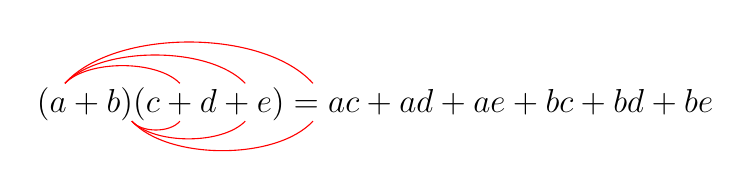
\begin{tikzpicture}
\draw node[right] {\large $(a+b)(c+d+e) = ac+ad+ae+bc+bd+be$};

\pgfmathsetmacro{\klAx}{0.48}
\pgfmathsetmacro{\klBx}{1.33}
\pgfmathsetmacro{\klCx}{1.94}
\pgfmathsetmacro{\klDx}{2.77}
\pgfmathsetmacro{\klEx}{3.63}
\pgfmathsetmacro{\klLo}{-0.22}
\pgfmathsetmacro{\klHi}{0.26}

\pbezier{\klAx}{\klCx}{\klHi}{0.3}
\pbezier{\klAx}{\klDx}{\klHi}{0.48}
\pbezier{\klAx}{\klEx}{\klHi}{0.7}

\pbezier{\klBx}{\klCx}{\klLo}{-0.15}
\pbezier{\klBx}{\klDx}{\klLo}{-0.3}
\pbezier{\klBx}{\klEx}{\klLo}{-0.5}
\end{tikzpicture}

Esimerkiksi polynomien $x-3$ ja $x^2-4x+3$ tulo voidaan laskea vastaavasti:

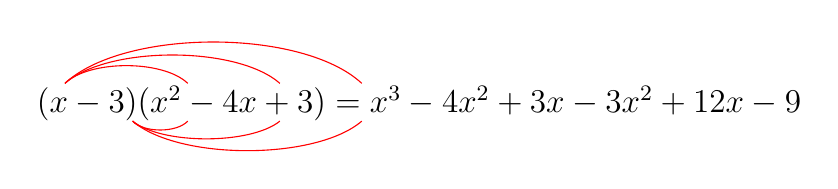
\begin{tikzpicture}
\draw node[right] {\large $(x-3)(x^2-4x+3) = x^3-4x^2+3x-3x^2+12x-9$};

\pgfmathsetmacro{\klAx}{0.48}
\pgfmathsetmacro{\klBx}{1.34}
\pgfmathsetmacro{\klCx}{2.04}
\pgfmathsetmacro{\klDx}{3.21}
\pgfmathsetmacro{\klEx}{4.25}
\pgfmathsetmacro{\klLo}{-0.22}
\pgfmathsetmacro{\klHi}{0.26}

\pbezier{\klAx}{\klCx}{\klHi}{0.3}
\pbezier{\klAx}{\klDx}{\klHi}{0.48}
\pbezier{\klAx}{\klEx}{\klHi}{0.7}

\pbezier{\klBx}{\klCx}{\klLo}{-0.15}
\pbezier{\klBx}{\klDx}{\klLo}{-0.3}
\pbezier{\klBx}{\klEx}{\klLo}{-0.5}
\end{tikzpicture}


Sievennetyksi vastaukseksi saadaan siis $x^3-7x^2+15x-9$.

\begin{esimerkki}
\begin{align*}
&\hspace{0.5cm}(x^4-3x^3+3)(x^3-2x^2+1) \\
&= x^4 (x^3-2x^2+1) - 3x^3 (x^3-2x^2+1) + 3 (x^3-2x^2+1) \\
&= x^4\cdot x^3 + x^4\cdot (-2x^2)+x^4\cdot 1-3x^3\cdot x^3-3x^3(-2x^2)-3x^3\cdot1+3x^3+3(-2x^2)+3\cdot 1 \\
&= x^7-2x^6+x^4-3x^6+6x^5-3x^3+3x^3-6x^2+3 \\
&= x^7-5x^6+6x^5+x^4-6x^2+3
\end{align*}
\end{esimerkki}

\section{Muistikaavat}

Eräitä polynomien kertolaskuja tarvitaan niin usein, että niitä kutsutaan muistikaavoiksi.

\laatikko{
    Muistikaavat
    \begin{itemize}
        \item $(a+b)^2 = a^2+2ab+b^2$
        \item $(a-b)^2 = a^2-2ab+b^2$
        \item $(a+b)(a-b) = a^2-b^2$
    \end{itemize}
}

Nämä kaavat voidaan helposti todistaa laskemalla.

\subsubsection*{Summan neliö}

\begin{align*}
(a+b)^2 &= (a+b)(a+b) &\emph{neliön määritelmä} \\
&= a(a+b)+b(a+b) &\emph{osittelulaki} \\
&= a^2+ab+ba+b^2 &\emph{osittelulaki} \\
&= a^2+ab+ab+b^2 &\emph{reaaliluvuille $ba=ab$} \\
&= a^2+2ab+b^2
\end{align*}

\subsubsection*{Erotuksen neliö}

\begin{align*}
(a-b)^2 &= (a-b)(a-b) &\emph{neliön määritelmä} \\
&= a(a-b)-b(a-b) &\emph{osittelulaki} \\
&= a^2-ab-ba+b^2 &\emph{osittelulaki} \\
&= a^2-ab-ab+b^2 &\emph{reaaliluvuille $ba=ab$} \\
&= a^2-2ab+b^2
\end{align*}

\subsubsection*{Summan ja erotuksen tulo}

\begin{align*}
(a+b)(a-b) &= a(a-b)+b(a-b) &\emph{osittelulaki} \\
&= a^2-ab+ba-b^2 &\emph{osittelulaki} \\
&= a^2-ab+ab-b^2 &\emph{reaaliluvuille $ba=ab$} \\
&= a^2-b^2
\end{align*}

\laatikko{
    Esimerkkejä
    \begin{itemize}
        \item $(3x+2y)^2 = (3x+2y)(3x+2y) = 9x^2+2\cdot 3x\cdot 2y+4y^2 = 9x^2+12xy+4y^2$
        \item $995^2 = (1000-5)^2 = 1000^2-2\cdot 1000\cdot 5+5^2 = 1000000-10000+25 = 990025$
        \item $104\cdot 96 = (100+4)(100-4) = 100^2 - 4^2 = 10000 - 16 = 9984$
    \end{itemize}
    }

\section{Tekijöihinjako}

Matematiikan 1. kurssilla on käsitelty lukujen jakamista tekijöihin.
Esimerkiksi luvun $12$ {\bf tekijät} ovat $1$, $2$, $3$, $4$, $6$ ja $12$. Nämä ovat sellaisia
lukuja, joista saadaan $12$ kertomalla ne jollain kokonaisluvulla. Sanotaan myös, että luvun $12$
{\bf alkutekijät} ovat $2$, $2$ ja $3$, koska luku $12$ voidaan
ilmaista niiden tulona ($2\cdot 2\cdot 3 = 2^2\cdot 3 = 12$), mutta näitä tekijöitä ei
voi enää jakaa pienempiin osatekijöihin. Kokonaisluvun tekijät ovat aina kokonaislukuja.

Vastaavasti voidaan puhua polynomin jakamisesta \termi{tekijöihin} tai
\termi{alkutekijöihin}. Polynomin tekijät
ovat aina polynomeja. Olemme jo oppineet kertomaan polynomeja keskenään,
joten voimme helposti laskea, että $(x-3)(2x^2-8x+8)=2x^3-14x^2+32x-24$.
Nyt voidaan sanoa, että $x-3$ ja $2x^2-8x+8$ ovat polynomin $2x^3-14x^2+32x-24$ tekijöitä.
Mutta ovatko ne alkutekijöitä, vai voidaanko ne edelleen jakaa pienempiin tekijöihin?
Itse asiassa laskemalla voidaan todeta että $2x^2-8x+8$ saadaan tulokseksi kertolaskusta $2(x-2)(x-2)=2(x-2)^2$.
Voimme siis ilmoittaa polynomin tekijöidensä avulla: $2x^3-14x^2+32x-24=2(x-3)(x-2)^2$.

Polynomin tekijöitä voi etsiä soveltamalla kertolaskua käänteisesti:

\begin{itemize}
\item Otetaan korkeimman asteen termin kerroin yhteiseksi tekijäksi: \\
$5x^4+3x^2+x-9 = 5(x^4+\frac{3}{5} x^2+\frac{1}{5} x-\frac{9}{5}$
\item Otetaan $x$ tai sen potenssi yhteiseksi tekijäksi, jos mahdollista: \\
$x^5+x^3+3x^2 = x^2(x^3+x+3)$
\item Sovelletaan muistikaavaa käänteisesti \\
$x^2-5=x^2-\sqrt{5}^2=(x+\sqrt{5})(x-\sqrt{5})$ \\
$x^2+8+16=x^2+2\cdot 4+4^2=(x+4)^2$ \\
$x^2+1+\frac14=x^2+2\cdot \frac12+(\frac12)^2=(x-\frac12)^2$
\end{itemize}

\begin{esimerkki}
Jaetaan tekijöihin polynomi $10x^3-20x^2$.

\begin{align*}
& 10x^3-20x^2 \\
=& 10(x^3-2x^2) \ \ \ \ &\emph{otetaan $10$ yhteiseksi tekijäksi} \\
=& 10x^2(x-2) &\emph{otetaan $x^2$ yhteiseksi tekijäksi} \\
\end{align*}
\end{esimerkki}

\begin{esimerkki}
Jaetaan tekijöihin polynomi $5x^3-20x^2+20x$.

\begin{align*}
& 5x^3-20x^2+20x \\
=& 5(x^3-4x^2+4x) \ \ \ \ &\emph{otetaan $5$ yhteiseksi tekijäksi} \\
=& 5x(x^2-4x+4) &\emph{otetaan $x$ yhteiseksi tekijäksi} \\
=& 5x(x^2-2\cdot 2x+2^2) \\
=& 5x(x-1)^2 &\emph{sovelletaan muistikaavaa} \\
\end{align*}
\end{esimerkki}

\begin{esimerkki}
Jaetaan tekijöihin polynomi $5x^7-2\sqrt{15}x^5+3x^3$.

\begin{align*}
& 5x^7-2\sqrt{15}x^5+3x^3 \\
=& 5\left(x^7-\frac{2\sqrt{15}}{5}x^5+\frac{3}{5}x^3\right) \ \ \ \ &\emph{otetaan $5$ yhteiseksi tekijäksi} \\
=& 5\left(x^7-2\sqrt{\frac35}x^5+\frac{3}{5}x^3\right) \\
=& 5x^3\left(x^4-2\sqrt{\frac35}x^2+\frac{3}{5}\right) &\emph{otetaan $x^3$ yhteiseksi tekijäksi} \\
=& 5x^3\left((x^2)^2-2\cdot x^2\cdot \sqrt{\frac35}+\sqrt{\frac35}^2\right) & \\
=& 5x^3\left(x^2-\sqrt{\frac35}\right)^2 &\emph{sovelletaan muistikaavaa} \\
=& 5x^3\left(x^2-\sqrt[4]{\frac35}^2\right)^2 \\
=& 5x^3\left(\left(x-\sqrt[4]{\frac35}\right)\left(x+\sqrt[4]{\frac35}\right)\right)^2 &\emph{sovelletaan muistikaavaa} \\
=& 5x^3\left(x-\sqrt[4]{\frac35}\right)^2\left(x+\sqrt[4]{\frac35}\right)^2 \\
\end{align*}
\end{esimerkki}

Kaikkien polynomien tekijöihinjako ei kuitenkaan näillä menetelmillä onnistu.
Myöhemmin tässä kirjassa opitaan, miten minkä tahansa polynomin voi jakaa tekijöihin nollakohtiensa avulla.

\section{Harjoitustehtäviä}

\begin{tehtava}
    Sievennä
    \begin{enumerate}[a)]
        \item $x(x^2 + 1)$
        \item $(x - 5)3x$
        \item $(-2x)(4x - 1)3$
        \item $2x(x + y)$
        \item $(3x^5 + 7)y$
        \item $(-x^3)(10x - 2)$
        \item $5(-2x + 1)(-9x) $
    \end{enumerate}
    \begin{vastaus}
        \begin{enumerate}[a)]
            \item $x^3 + x$
            \item $3x^2 - 15x$
            \item $-24x^2 + 6x$
            \item $2x^2 + xy$
            \item $3x^5y + 7y$
            \item $-10x^4 + 2x^3$
            \item $90x^2 - 45x$
        \end{enumerate}
    \end{vastaus}
\end{tehtava}

\begin{tehtava}
    Sievennä
    \begin{enumerate}[a)]
        \item $(x+2)^2$
        \item $(x-3)^2$
        \item $(x-1)(x+1)$
        \item $(5-x)^2$
        \item $(2x + 8)^2$
        \item $(9 - 7x)(9 + 7x)$
    \end{enumerate}
    \begin{vastaus}
        \begin{enumerate}[a)]
            \item $x^2 + 4x + 4$
            \item $x^2 - 6x + 9$
            \item $x^2 - 1$
            \item $x^2 - 10x + 25$
            \item $4x^2 + 32x + 64$
            \item $-49x^2 + 81$
        \end{enumerate}
    \end{vastaus}
\end{tehtava}

\begin{tehtava}
    Sievennä
    \begin{enumerate}[a)]
        \item $(t+v)^2+(t-v)^2$
        \item $(t+v)^2-(t-v)^2$
    \end{enumerate}
    \begin{vastaus}
        \begin{enumerate}[a)]
            \item $(t+v)^2+(t-v)^2 = t^2+2tv+v^2+t^2-2tv+v^2 = 2t^2+2v^2$
            \item $(t+v)^2-(t-v)^2 = t^2+2tv+v^2-t^2+2tv-v^2 = 4tv$
        \end{enumerate}
    \end{vastaus}
\end{tehtava}

\begin{tehtava}
    Sievennä (vinkki: käytä summakaavoja)
    \begin{enumerate}[a)]
        \item $63^2+37^2$
        \item $101^2+99^2$
    \end{enumerate}
    \begin{vastaus}
        \begin{enumerate}[a)]
            \item $63^2+37^2 = (50+13)^2+(50-13)^2 = 2\cdot 50^2 + 2\cdot 13^2 = 2\cdot 2500 +2\cdot 169 = 5000 + 338 = 5338$
            \item $101^2+99^2 = (100+1)^2+(100-1)^2 = 2\cdot 100^2 + 2\cdot 1^2 = 2\cdot 10000 + 2\cdot 1 = 20000 + 2 = 20002$
        \end{enumerate}
    \end{vastaus}
\end{tehtava}

\begin{tehtava}
    Sievennä
    \begin{enumerate}[a)]
        \item $35^2-25^2$
        \item $170^2-50^2$
    \end{enumerate}
    \begin{vastaus}
        \begin{enumerate}[a)]
            \item $35^2-25^2 = (30+5)^2-(30-5)^2 = 4\cdot 30\cdot 5 = 600$
            \item $170^2-30^2 = (100+70)^2+(100-70)^2 = 4\cdot 100\cdot 70 = 28000$
        \end{enumerate}
    \end{vastaus}
\end{tehtava}

\begin{tehtava}
    Sievennä
    \begin{enumerate}[a)]
        \item $(x+1)(x+3)$
        \item $(x+2)(x-1)$
        \item $(2x+5)(x+7)$
        \item $(x-1)(x+4)x$
    \end{enumerate}
    \begin{vastaus}
        \begin{enumerate}[a)]
            \item $x^2 + 4x + 3$
            \item $x^2 + x - 2$
            \item $2x^2 + 19x + 35$
            \item $x^3 + 3x^2 - 4x$
        \end{enumerate}
    \end{vastaus}
\end{tehtava}

\begin{tehtava}
    Johda ''muistikaavat'' potenssien
    \begin{enumerate}[a)]
            \item $(a+b)^3$
            \item $(a+b)^4$
            \item $(a-b)^3$
        \end{enumerate}
        aukikertomiseksi.
    \begin{vastaus}
        \begin{enumerate}[a)]
            \item $(a+b)^3 = a^3 + 3a^2b + 3ab^2 + b^3$
            \item $(a+b)^4 = a^4 + 4a^3b + 6a^2b^2 + 4ab^3 + b^4$
            \item $(a-b)^3 = a^3 - 3a^2b + 3ab^2 - b^3$
        \end{enumerate}
    \end{vastaus}
\end{tehtava}

\begin{tehtava}
	Laske polynomien kertolaskut
	\begin{enumerate}[a)]
		\item $(x-3)(2x^3-3x+4)$
		\item $(x^2+1)(x^3-2x-4)$
		\item $(x-1)(x^4+x^3+x^2+x+1)$
		\item $(\frac x5-\frac23)(x^2+x+1)$
	\end{enumerate}
	\begin{vastaus}
		\begin{enumerate}[a)]
			\item $2x^4-6x^3-3x^2+13x-12$
			\item $x^5-x^3-4x^2-2x-4$
			\item $x^5-1$
			\item $\frac15x^3-\frac{7}{15}x^2-\frac{7}{15}x-\frac23$
		\end{enumerate}
	\end{vastaus}
\end{tehtava}

	%polynomin kertominen monomilla a(x+b)=ax+ab
	%kahden binomin tulo: (a+b)(c+d)=ac+ad+bc+bd
	%tekijöihin jako, käsite tekijä
	%muistikaavat
		%(a+b)^2=a^2+2ab+b^2
		%(a-b)^2=a^2-2ab+b^2
		%(a-b)(a+b)=a^2-b^2
		%Esimerkki tai harjoitustehtävä: 102*98=(100+2)(100-2)=10000-4
	\section{Tekijöihinjako}

\qrlinkki{http://opetus.tv/maa/maa2/polynomin-jakaminen-tekijoihin/}{Opetus.tv: \emph{polynomin jakaminen tekijöihin} (9:50 ja 5:44)}


%Pitkän matematiikan 1. kurssilla on käsitelty lukujen jakamista tekijöihin.
Esimerkiksi luvun $12$ \termi{tekijä}{tekijät} ovat luvut $1$, $2$, $3$, $4$, $6$ ja $12$. Nämä ovat sellaisia
lukuja, joista saadaan luku $12$ kertomalla ne jollain kokonaisluvulla, tai toisin sanottuna luku $12$ voidaan jakaa
millä tahansa näistä luvuista ilman jakojäännöstä.
%Sanotaan myös, että luvun $12$ \termi{alkutekijä}{alkutekijät} ovat $2$ ja $3$, koska luku $12$ voidaan
%ilmaista niiden tulona ($2\cdot 2\cdot 3 = 2^2\cdot 3 = 12$), mutta näitä tekijöitä ei
%voi enää jakaa pienempiin osatekijöihin. Kokonaisluvun tekijät ovat kokonaislukuja ja alkutekijät alkulukuja.

\begin{esimerkki}
Luku $12$ voidaan kirjoittaa tekijöidensä tulona monella eri tavalla. Esimerkiksi
\begin{align*}
&12 = 2 \cdot 6, \\
&12= 4 \cdot 3 \text{ tai } \\
&12= 2 \cdot 2 \cdot 3.
\end{align*}
\end{esimerkki}

Polynomeja voidaan jakaa vastaavalla tavalla tekijöihin. Polynomien tapauksessa tekijöihinjako tarkoittaa
polynomin esittämistä saman- tai pienempiasteisten polynomien tulona. Aste on aina pienempi, ellei kyse ole pelkästä
vakiokertoimen ottamisesta yhteiseksi tekijäksi.

\begin{esimerkki}
Jaa tekijöihin polynomi $10x^3-20x^2$.
\begin{align*}
& 10x^3-20x^2 \\
=& 10(x^3-2x^2) \ \ \ \ &\emph{otetaan $10$ yhteiseksi tekijäksi} \\
=& 10x^2(x-2) &\emph{otetaan $x^2$ yhteiseksi tekijäksi} \\
\end{align*}
\end{esimerkki}

\begin{esimerkki}
Jaa tekijöihin \quad a) $x^3+x$ \quad b) $3x^2+6x.$

Kun jokaisessa termissä on sama tekijä, se voidaan ottaa yhteiseksi tekijäksi:
\begin{enumerate}[a)]
    \item $x^3+x = x(x^2+1)$
    \item $3x^2+6x = 3x(x+2)$.
\end{enumerate}
\end{esimerkki}

\begin{esimerkki}
Jaa tekijöihin polynomi $5x^3-20x^2+20x$.
\begin{align*}
& 5x^3-20x^2+20x \\
=& 5(x^3-4x^2+4x) \ \ \ \ &\emph{otetaan $5$ yhteiseksi tekijäksi} \\
=& 5x(x^2-4x+4) &\emph{otetaan $x$ yhteiseksi tekijäksi} \\
=& 5x(x^2-2\cdot 2x+2^2) &\emph{sovelletaan muistikaavaa} \\
=& 5x(x-2)^2
\end{align*}
\end{esimerkki}

\begin{esimerkki}
Jaa tekijöihin \quad a) $x^2-4$ \quad b) $x^2+8x+16.$

Jaetaan polynomit tekijöihin hyödyntämällä muistikaavoja
\begin{enumerate}[a)]
    \item $x^2-4 = x^2-2^2 = (x+2)(x-2)$
    \item $x^2+8x+16 = x^2+ 2\cdot 4 \cdot x + 4^2 = (x+4)^2$
\end{enumerate}
\end{esimerkki}

%On suositeltavaa tarkistaa itse, että yllä esitetyt tekijöihinjaot todella toimivat. Polynomien tekijöihinjaon toimivuus
%on helppoa tarkistaa -- täytyy vain laskea väitettyjen tekijöiden tulo ja katsoa, onko se alkuperäinen polynomi. Vaikka
%tarkistus onkin helppoa, tässä vaiheessa ei luultavasti vielä ole selvää, miten tekijöihinjaon voisi saada selville
%-- paitsi toisinaan arvaamalla, mutta tähän kysymykseen vastataan myöhemmin tällä kurssilla.

%Polynomien tekijöihinjako ei ole yksiselitteinen, mutta monesti hyödyllisintä on jakaa polynomi tekijöihin samoin kuin
%esimerkkitapauksissa eli niin, että ensimmäisenä on vakiotermi ja kaikissa muissa tekijäpolynomeissa korkeimman asteen
%termin kerroin on 1.
%
%Esimerkki selkeyttänee asiaa. Polynomi $6x^2+30x+36$ voidaan jakaa tekijöihin vaikkapa seuraavilla tavoilla:
%
%\begin{esimerkki}
%\qquad \\
%\begin{itemize}
%    \item $6(x+2)(x+3)$
%    \item $3(2x+4)(x+3)$
%    \item $3(x+2)(2x+6)$
%    \item $2(3x+6)(x+2)$
%    \item $(6x+12)(x+3)$
%    \item $(\frac12 x+1)(12x+36)$
%\end{itemize}
%\end{esimerkki}
%
%Kaikki nämä tavat ovat ''oikein,'' mutta lähes aina ensimmäinen muoto $6(x+2)(x+3)$ on kätevin.
%
%Toisinaan polynomeille voi löytää tekijöitä soveltamalla joitakin seuraavista keinoista:
%
%\begin{itemize}
%\item Otetaan korkeimman asteen termin kerroin yhteiseksi tekijäksi: \\
%$5x^4+3x^2+x-9 = 5(x^4+\frac{3}{5} x^2+\frac{1}{5} x-\frac{9}{5})$
%\item Otetaan $x$ tai sen potenssi yhteiseksi tekijäksi, jos mahdollista: \\
%$x^5+x^3+3x = x(x^4+x^2+3)$
%$x^7+x^6+5x^4+2x^2 = x^2(x^5+x^4+5x^2+2)$
%\item Sovelletaan muistikaavaa käänteisesti \\
%$x^2-5=x^2-\sqrt{5}^2=(x+\sqrt{5})(x-\sqrt{5})$ \\
%$x^2+8x+16=x^2+2\cdot 4x+4^2=(x+4)^2$ \\
%$x^2+x+\frac14=x^2+2\cdot \frac12 x+(\frac12)^2=(x+\frac12)^2$
%\end{itemize}

Kaikkien polynomien tekijöihinjako ei kuitenkaan näillä menetelmillä onnistu. Myöhemmin tässä kirjassa opitaan, miten toisen asteen polynomin voidaan jakaa tekijöihin nollakohtiensa avulla.

Seuraavassa esimerkissä tekijöihin jako on toteutettu termien ryhmittelyn avulla. Se on joissain tapauksissa näppärä tapa jakaa polynomi tekijöihin, mutta oikean ryhmittelyn keksimiseen ei ole mitään sääntöä.

\begin{esimerkki}
Jaa tekijöihin $x^3+3x^2+x+3$.
\begin{equation*}
x^3+3x^2+x+3=x^2(x+3)+1(x+3)=(x^2+1)(x+3)
\end{equation*}
\end{esimerkki}

\begin{esimerkki}
Jaa tekijöihin $x^{11}+2x^{10}+3x+6$.
\begin{align*}
& x^{11}+2x^{10}+3x+6=x^{10}(x+2)+3(x+2)=(x^{10}+3)(x+2)
\end{align*}
\end{esimerkki}

\begin{tehtavasivu}

\paragraph*{Opi perusteet}

\begin{tehtava}
    Esitä tulona ottamalla yhteinen tekijä.
    \begin{enumerate}[a)]
        \item $2x+6$
        \item $x^2 -4x$
        \item $3x^2 - 6x$
    \end{enumerate}
    \begin{vastaus}
        \begin{enumerate}[a)]
        \item $2(x+3)$
        \item $x(x-4)$
        \item $3x(x-2)$
        \end{enumerate}
    \end{vastaus}
\end{tehtava}

\begin{tehtava}
    Jaa tekijöihin.
    \begin{enumerate}[a)]
        \item $-15^5 +10y$
        \item $x^3y^2 +x^2y^3$
        \item $-4a^3 -2a^2 +2ab$
    \end{enumerate}
    \begin{vastaus}
        \begin{enumerate}[a)]
        \item joko $5(-3x^5 +2y)$ tai $-5(3x^5 -2y)$
        \item $x^2y^2(x+y)$
        \item joko $2a(-2a^2 -a +b)$ tai $-2a(2a^2 +a -b)$
        \end{enumerate}
    \end{vastaus}
\end{tehtava}

\begin{tehtava}
    Jaa tekijöihin.
    \begin{enumerate}[a)]
        \item $x^2+6x+9$
        \item $y^2 - 2y+1$
        \item $x^2 -25$
    \end{enumerate}
    \begin{vastaus}
        \begin{enumerate}[a)]
        \item $(x+3)^2$
        \item $(y-1)^2$
        \item $(x-5)(x+5)$
        \end{enumerate}
    \end{vastaus}
\end{tehtava}

\begin{tehtava}
    Jaa tekijöihin.
    \begin{enumerate}[a)]
        \item $4x^2 +4x +1$
        \item $4x^2 +4x +4$
        \item $9-x^2$
          \end{enumerate}
    \begin{vastaus}
        \begin{enumerate}[a)]
        \item $(2x+1)^2$
        \item $4(x^2 +x +1)$
        \item $(3+x)(3-x)$
        \end{enumerate}
    \end{vastaus}
\end{tehtava}

\begin{tehtava}
    Jaa tekijöihin.
    \begin{enumerate}[a)]
        \item $x^3 +x^2 +x +1$
        \item $a^3 +a^2b +2a +2b$
        \item $4m^5 -2m^3 +2m^2 -1$
    \end{enumerate}
    \begin{vastaus}
        \begin{enumerate}[a)]
        \item $(x^2+1)(x+1)$
        \item $(a^2+2)(a+b)$
        \item $(2m^3 -1)(2m^2 -1)$
        \end{enumerate}
    \end{vastaus}
\end{tehtava}

\paragraph*{Hallitse kokonaisuus}

\begin{tehtava}
    Jaa tekijöihin.
    \begin{enumerate}[a)]
    	\item $x^3 - x$
        \item $x^2 - x + \frac{1}{4} $
        \item $9-x^4$
    \end{enumerate}
    \begin{vastaus}
        \begin{enumerate}[a)]
            \item $x(x-1)^2$
            \item $(x-\frac{1}{2})^2$
            \item $(3+x^2)(3-x^2)$
        \end{enumerate}
    \end{vastaus}
\end{tehtava}

\begin{tehtava}
    Jaa tekijöihin.
    \begin{enumerate}[a)]
    	\item $x^2 -4$
    	\item $x^2 -3$
    	\item $5x^2 -3$
    \end{enumerate}
    \begin{vastaus}
        \begin{enumerate}[a)]
            \item $(x+2)(x-2)$
            \item $(x+\sqrt{3})(x-\sqrt{3})$
            \item $(\sqrt{5}x+\sqrt{3})(\sqrt{5}x-\sqrt{3})$
        \end{enumerate}
    \end{vastaus}
\end{tehtava}

\paragraph*{Lisää tehtäviä}

\end{tehtavasivu}

	\chapter{Tulon nollasääntö ja tulon merkkisääntö}
	%tulon nollasääntö
		%tulo on 0 jos ja vain jos ainakin yksi tulon tekijöistä on 0
		%esim. yhtälön x(x-2)=0 ratkaisu
		%korostetaan lyhyesti, että kyseessä on reaalilukujen ominaisuus, joka ei kaikissa muissa joukoissa välttämättä päde
		%liitteeseen voi ajan riittäessä laittaa eksplisiittisen esimerkin tällaisesta joukosta
	%tulon merkkisääntö
		%positiivinen * positiivinen = positiivinen
		%positiivinen * negatiivinen = negatiivinen
		%negatiivinen * negatiivinen = positiivinen
		%sovellus: x^2>=0
	%on hyvä mainita, että säännöt voidaan todistaa
	%todistukset korkeintaan liitteeksi
	\chapter{Polynomifunktion kuvaaja}
Polynomifunktioita on monesti hyödyllistä
havainnollistaa koordinaatistoon piirrettynä kuvaajana.
%Tavallisesti $xy$-koordinaatistossa pystyakselin arvot eli korkeus vastaavat
%funktion arvoja,
%joten polynomin $P$ kuvaaja on siis sama asia kuin käyrän $y = P(x)$.

Nämä kuvaajat voisi piirtää eri koordinaatistoihin.

\begin{kuvaajapohja}{1.5}{-2}{2}{-3}{3}
\kuvaaja{-x-1}{$P(x) = -x-1$}{red}
\kuvaaja{x**2+x}{$Q(x) = x^2+x$}{blue}
\kuvaaja{x**3-3*x-1}{$R(x) = x^3-3x-1$}{green}
\end{kuvaajapohja}


\section*{Kuvaajan piirtäminen}

Funktion kuvaajien piirtäminen käsin onnistuu yleensä helpoiten laskemalla
funktion arvoja muutamilla muuttujan arvoilla, merkitsemällä pisteet
$xy$-koordinaatistoon ja hahmottamalla pisteiden kautta kulkeva kuvaaja.

\begin{esimerkki}
Hahmotellaan polynomifunktion $f(x) = \dfrac{1}{2}x^2 - x - 2$ kuvaaja.
Lasketaan ensin joitakin funktion $f(x) = \dfrac{1}{2}x^2 - x - 2$ arvoja ja piirretään niitä vastaavat pisteet
koorinaatistoon. Lopuksi hahmotellan kuvaaja, joka kulkee pisteiden kautta.

\begin{tabular}{c c c}
	\begin{tabular}{|c|r @{,} l|}
	\hline $x$ & \multicolumn{2}{c|}{$f(x)$} \\
	\hline
	-3 & 5&5 \\
	-2 & 2&0 \\
	-1 & -0&5 \\
	0 & -2&0 \\
	1 & -2&5 \\
	2 & -2&0 \\
	3 & -0&5 \\
	\hline
	\end{tabular}
	&
	\vcent{\begin{kuvaajapohja}{0.6}{-4}{4}{-3}{6}
	\kuvaajapiste{-3}{5.5}
	\kuvaajapiste{-2}{2}
	\kuvaajapiste{-1}{-0.5}
	\kuvaajapiste{0}{-2}
	\kuvaajapiste{1}{-2.5}
	\kuvaajapiste{2}{-2}
	\kuvaajapiste{3}{-0.5}
	\end{kuvaajapohja}}
	&
	\vcent{\begin{kuvaajapohja}{0.6}{-4}{4}{-3}{6}
	\kuvaajapiste{-3}{5.5}
	\kuvaajapiste{-2}{2}
	\kuvaajapiste{-1}{-0.5}
	\kuvaajapiste{0}{-2}
	\kuvaajapiste{1}{-2.5}
	\kuvaajapiste{2}{-2}
	\kuvaajapiste{3}{-0.5}
	\kuvaaja{0.5*x**2-x-2}{$f(x) = \dfrac{1}{2}x^2 - x - 2$}{red}
	\end{kuvaajapohja}}
\end{tabular}

\end{esimerkki}

\section*{Kuvaajan tulkintaa}

%Ensimmäisen asteen polynomin kuvaaja on luonnollisesti aina suora. 
%miten niin luonnollisesti?

Kuvaajan avulla voidaan tehdä johtopäätöksiä funktion ominaisuuksista.
Esimeriksi funktion arvoja voidaan lukea kuvaajasta.

\begin{esimerkki}
Alla on esitetty erään polynomifunktion $P(x)$ kuvaaja. Kuvaajan perusteella näyttäisi siltä, että $P(1)=(-1)$,
mutta tarkkaa arvoa kuvaajasta ei voi päätellä.

\begin{kuvaajapohja}{1}{-2}{2}{-2}{2}
\kuvaaja{x**4-2*x**3-x**2+11./10}{P(x)}{red}
\end{kuvaajapohja}

Itse asiassa edellinen kuvaaja on funktion $P(x)=x^4-2x^3-x^2+\dfrac{11}{10}$ kuvaaja.
Siten $P(1)=-\dfrac{9}{10}$ eikä $-1$ kuten kuvaajan perusteella voisi luulla.
\end{esimerkki}

Funktion nollakohta on sellainen muuttujan arvo, jolla funktio saa arvon nolla. Esimerkiksi funktiolla $Q(x)=x^2-1$
on nollakohdat $-1$ ja $1$, sillä $Q(1)=0$ ja $Q(-1)=0$. Polynomien tapauksessa nollakohtia on tapana kutsua
\termi[juuriksi]{juuri, polynomin}.

Funktion kuvaaja antaa tietoa nollakohdista. Niiden kohdalla kuvaaja leikkaa $x$-akselin.

\begin{esimerkki}
Funktion $Q(x) = x^2-1$ kuvaajasta nähdään, että funktiolla on kaksi nollakohtaa, $1$ ja $-1$.

\begin{kuvaajapohja}{1}{-2}{2}{-2}{4}
\kuvaaja{x**2-1}{$Q(x) = x^2-1$}{red}
\end{kuvaajapohja}
\end{esimerkki}

%Nollakohta tarkoittaa sitä annetun polynomin muuttujan arvoa, jolla koko
%polynomi saa arvon nolla. Kuvaajasta sen voi helposti lukea niinä kohtina,
%joissa kuvaaja leikkaa muuttujan koordinaattiakselin. Funktion $P(x)$ ja
%$xy$-koordinaatiston tapauksessa funktion nollakohdat ovat täsmälleen ne
%$x$-koordinaatit, joilla funktion kuvaaja leikkaa $x$-akselin.

%\section{Taylorin sarja}
%Eräs mielenkiintoinen ja hyvin tunnettu potenssisarja on Taylorin sarja.
%Se on päättymätön potenssisarja, jolla voidaan approksimoida muiden funktioiden
%arvoja.
%
%Yleisesti Taylorin sarjalla saadaan (rajatta derivoituvan) funktion $f$ arvo
%pisteessä $x_0$:
%
%\begin{align*}
%	f(x_0) = \sum\limits_{n=0}^\infty a_n(x-x_0)^n
%\end{align*}
%
%missä
%
%\begin{align*}
%a_n = \frac{f^n(x_0)}{n!}
%\end{align*}
%
%Koska sarja on äärettömän pitkä, sarjan arvoja edelleen arvioidaan Taylorin
%polynomilla, joka on muotoa
%
%\begin{align*}
%	P_k(x) = \sum\limits_{n=0}^k a_k(x-x_0)^k
%\end{align*}
%
%Polynomin avulla voidaan laskea esimerkiksi likiarvo funktiolle
%$(1-x)^{-1} = \frac{1}{1-x}$ pisteen a ympäristössä, kun $a \neg 1$:
%
%\begin{align*}
%	\frac{1}{1-x} \approx \frac{1}{1-a} + \frac{x-a}{(1-a)^2} +
%\frac{(x-a)^2}{(1-a)^3} + \frac{(x-a)^3}{(1-a)^4} ...
%\end{align*}
%
%\missingfigure{Funktion $(x-1)^-1$ kuvaaja}
%\missingfigure{Funktion $\frac{1}{1-a} + \frac{x-a}{(1-a)^2} +
%\frac{(x-a)^2}{(1-a)^3} +$ kuvaaja}

\Harjoitustehtavat

\begin{tehtava}
    Piirrä polynomien kuvaajat.
    \begin{enumerate}[a)]
        \item $5$
        \item $2x-3$
        \item $x^2+x-2$
        \item $x^3-x+3$
    \end{enumerate}   
    \begin{vastaus}
    	\item \begin{kuvaajapohja}{0.4}{-4}{4}{-1}{7}
				\kuvaaja{5}{}{red}
			  \end{kuvaajapohja}
    	\item \begin{kuvaajapohja}{0.4}{-4}{4}{-5}{3}
				\kuvaaja{2*x-3}{}{red}
			  \end{kuvaajapohja}
		\item \begin{kuvaajapohja}{0.4}{-4}{4}{-3}{5}
				\kuvaaja{x**2+x-2}{}{red}
			  \end{kuvaajapohja}
		\item \begin{kuvaajapohja}{0.4}{-4}{4}{-3}{5}
				\kuvaaja{x**3-x+2}{}{red}
			  \end{kuvaajapohja}
    \end{vastaus}
\end{tehtava}

\begin{tehtava}
    Piirrä polynomien kuvaajat.
    \begin{enumerate}[a)]
        \item $x+4$
        \item $2x-9$
        \item $5x+2$
        \item $6x+1$
    \end{enumerate}
    \begin{vastaus}
        \item \begin{kuvaajapohja}{0.4}{-4}{4}{-1}{7}
				\kuvaaja{x+4}{}{red}
			  \end{kuvaajapohja}
    	\item \begin{kuvaajapohja}{0.4}{-2}{6}{-6}{2}
				\kuvaaja{2*x-9}{}{red}
			  \end{kuvaajapohja}
		\item \begin{kuvaajapohja}{0.4}{-4}{4}{-2}{6}
				\kuvaaja{5*x+2}{}{red}
			  \end{kuvaajapohja}
		\item \begin{kuvaajapohja}{0.4}{-4}{4}{-2}{6}
				\kuvaaja{6*x+1}{}{red}
			  \end{kuvaajapohja}
    \end{vastaus}
\end{tehtava}

\begin{tehtava}
    Piirrä polynomien kuvaajat.
    \begin{enumerate}[a)]
        \item $x^2-1$
        \item $2x^2$
        \item $4x^2+4$
        \item $x^2-6x+3$
    \end{enumerate}
    \begin{vastaus}
        \item \begin{kuvaajapohja}{0.4}{-4}{4}{-2}{6}
				\kuvaaja{x+4}{}{red}
			  \end{kuvaajapohja}
    	\item \begin{kuvaajapohja}{0.4}{-4}{4}{-1}{7}
				\kuvaaja{2*x-9}{}{red}
			  \end{kuvaajapohja}
		\item \begin{kuvaajapohja}{0.4}{-4}{4}{-1}{11}
				\kuvaaja{5*x+2}{}{red}
			  \end{kuvaajapohja}
		\item \begin{kuvaajapohja}{0.4}{-1}{7}{-7}{5}
				\kuvaaja{6*x+1}{}{red}
			  \end{kuvaajapohja}
    \end{vastaus}
\end{tehtava}

\begin{tehtava}
    Piirrä polynomien kuvaajat.
    \begin{enumerate}[a)]
        \item $5x^2$
        \item $3x^2+4$
        \item $2x^2-10$
        \item $x^2-x-1$
    \end{enumerate}
    \begin{vastaus}
        \item \begin{kuvaajapohja}{0.4}{-4}{4}{-1}{7}
				\kuvaaja{5*x**2}{}{red}
			  \end{kuvaajapohja}
    	\item \begin{kuvaajapohja}{0.4}{-4}{4}{-1}{11}
				\kuvaaja{3*x**2+4}{}{red}
			  \end{kuvaajapohja}
		\item \begin{kuvaajapohja}{0.4}{-4}{4}{-11}{1}
				\kuvaaja{2*x**2-10}{}{red}
			  \end{kuvaajapohja}
		\item \begin{kuvaajapohja}{0.4}{-3}{5}{-2}{6}
				\kuvaaja{x**2-x-1}{}{red}
			  \end{kuvaajapohja}
    \end{vastaus}
\end{tehtava}

\begin{tehtava}
	Monia funktioita voidaan esittää likimääräisesti polynomeina (ns.
Taylorin polynomi). Esimerkiksi

	\begin{tabular}{lcll}
	$\frac{1}{1+x^2}$ &$\approx$ & $1-x^2+x^4-x^6+x^8-x^{10}$, & kun
$-1<x<1$ \\
	$\sqrt{1+x}$ & $\approx $ & $ 1+\frac{x}{2}
	-\frac{x^2}{8}+\frac{x^3}{16}-\frac{5x^4}{128}$, & kun $-1<x<1$
	\end{tabular}

	Piirrä alkuperäinen funktio ja polynomi samaan kuvaajaan tietokoneella
tai graafisella laskimella. Kokeile, kuinka polynomin viimeisten termien pois
jättäminen vaikuttaa tarkkuuteen. Mitä havaitset? (Termejä voi laskea lisääkin,
mutta siihen ei puututa tässä.)

	\begin{vastaus}
		Mitä enemmän termejä, sitä parempi vastaavuus.
	\end{vastaus}
\end{tehtava}

	%tarkoituksena varmistaa, että opiskelijat:
		%muistavat koordinaatiston idean
		%osaavat hahmotella funktion kuvaajan laskemalla sen arvoja
		%osaavat lukea funktion arvoja kuvaajasta sekä
		%oppivat käsitteen nollakohta
	%esimerkkeinä polynomeja
	%mitään yleistä teoriaa polynomien kuvaajista ei tarvita, mainittakoon että ensimmäisen asteen funktion kuvaaja on suora

\chapter{Ensimmäinen aste}
	%% encoding: utf-8
\section{Kertausta: Ensimmäisen asteen yhtälö}

Yhtälöistä yksinkertaisin on ensimmäisen asteen yhtälö. Käydään se lyhyesti
läpi kertauksen vuoksi.

Ensimmäisen asteen yhtälössä ratkaistavana on vain mahdollisesti vakiolla
kerrottu muuttuja. Yhtälön ratkaisemiseksi riittää käyttää neljää
aritmeettista peruslaskutoimitusta. Aluksi yhtälön molemmille puolille 
lisätään tai vähennetään jokin luku, niin että 
vasemmalle puolelle saadaan jäämään pelkkä vakiolla kerrottu muuttuja.
Sen jälkeen jaetaan yhtälön molemmat puolet muuttujan kertoimella, jolloin
yhtälön ratkaisu jää oikealle puolelle.

% fixme tyylikorjausta, termiä juuri ei vielä esitellä

Yleisesti ensimmäisen asteen yhtälö on muotoa

\begin{align*}
    ax + b = 0.
\end{align*}

Kaikki 1. asteen yhtälöt voidaan muokata tähän yleiseen
muotoon siirtämällä kaikki termit vasemmalle puolelle ja
sieventämällä.

% fixme Esimerkit 2.30-2.31 voisi siirtää ennen yleisen muodon esittelyä, koska niissä ei sitä mihinkään tarvita.

\subsubsection*{Esimerkkejä}

\begin{esimerkki}
Ratkaise yhtälö $4x + 5 = 2 + 2x$.

\textbf{Ratkaisu}
\begin{align*}
    4x + 5 &= 2 + 2x && \ppalkki -2x \\
    2x + 5 &= 2      && \ppalkki -5 \\
        2x &= -3     && \ppalkki :2 \\
         x &= -\frac{3}{2}
 \end{align*}
\end{esimerkki}

\begin{esimerkki}
Ratkaise yhtälö $3x - 6 = 0$.

\textbf{Ratkaisu}
  \begin{align*}
    3x - 6 &= 0 && \ppalkki +6 \\
        3x &= 6 && \ppalkki :3 \\
         x &= \frac{6}{3} \\
           &= 2
  \end{align*}
\end{esimerkki}

Yleisen yhtälön $ax + b = 0$ ratkaisu on siis

\begin{align*}
  x = -\frac{b}{a}.
\end{align*}

Erityisesti kannattaa huomata, että kaikkia 1. asteen yhtälöitä ei tarvitse
saattaa yleiseen muotoon. Esimerkiksi jos vakiotermit ovat valmiiksi
oikealla puolella, yhtälön ratkaisemiseksi riittää luonnollisesti jakaa
molemmat puolet muuttujan kertoimella.

\begin{tehtavasivu}

\paragraph*{Opi perusteet}

\begin{tehtava}
    Ratkaise yhtälöt.
    \begin{alakohdat}
        \alakohta{$x + 5 = 47$}
        \alakohta{$2x = 64$}
        \alakohta{$3x - 5 = 16$}
    \end{alakohdat}
    \begin{vastaus}
        \begin{alakohdat}
            \alakohta{$x = 42$}
            \alakohta{$x = 32$}
            \alakohta{$x = 7$}
        \end{alakohdat}
    \end{vastaus}
\end{tehtava}

\begin{tehtava}
    Ratkaise yhtälöt.
    \begin{alakohdat}
        \alakohta{$x + 8 = 2x - 1$}
        \alakohta{$2x + 4 = 60$}
        \alakohta{$3x - 5 = -x + 11$}
    \end{alakohdat}
    \begin{vastaus}
        \begin{alakohdat}
            \alakohta{$x = 9$}
            \alakohta{$x = 28$}
            \alakohta{$x = 4$}
        \end{alakohdat}
    \end{vastaus}
\end{tehtava}

%ei ole yhtälötehtävä, mutta mallinnusharjoituksena ok? 
\begin{tehtava}
    Muodosta tilannetta kuvaavat lausekkeet.
    \begin{alakohdat}
        \alakohta{Kuinka paljon maksaa hilavitkuttimen vuokraus $x$ tunniksi, kun vuokra on 42 \euro /tunti. }
        	Vuokraajan tulee myös ottaa pakollinen 25 euron laitteistovakuutus.
        \alakohta{Kuinka monta euroa saa $x$ dollarilla, kun 1~EUR vastaa 1,23~USD:a,}
        	ja halutaan vaihtaa dollareita euroiksi. Valuutanvaihtaja veloittaa lisäksi palvelumaksun 0,50 euroa.
    \end{alakohdat}
    \begin{vastaus}
        \begin{alakohdat}
            \alakohta{$42x + 25$}
            \alakohta{$\frac{1}{1{,}23}x + 0{,}5$}
        \end{alakohdat}
    \end{vastaus}
\end{tehtava}



\paragraph*{Hallitse kokonaisuus}

\begin{tehtava}
    Ratkaise yhtälöt.
    \begin{alakohdat}
        \alakohta{$3(x+7)=7x$}
        \alakohta{$2(3x-1)=-7x $}
        \alakohta{$3-2x-(4-x)=2 $}
    \end{alakohdat}
    \begin{vastaus}
        \begin{alakohdat}
            \alakohta{$x = \frac{7}{6} =1\frac{1}{6} $}
            \alakohta{$x = \frac{2}{13}$}
            \alakohta{$x = -3$}
        \end{alakohdat}
    \end{vastaus}
\end{tehtava}

\begin{tehtava}
    Ratkaise yhtälöt.
    \begin{alakohdat}
        \alakohta{$-2\cdot\frac{x-5}{3}-\frac{5}{7}(1-x)=5x+3$}
        \alakohta{$\frac{4x-5}{3}-\frac{3}{2}(x-8)=-\frac{x+5}{6}$}
        \alakohta{$3(x-3)+x=4x-9$}
    \end{alakohdat}
    \begin{vastaus}
        \begin{alakohdat}
            \alakohta{$x = -\frac{1}{13}$}
            \alakohta{ei ratkaisuja}
            \alakohta{yhtälö on toteutuu kaikilla reaaliluvuilla}
        \end{alakohdat}
    \end{vastaus}
\end{tehtava}

%vaatii Pythagoraan lauseen, jota ei vielä ole käsitelty lukiossa.
\begin{tehtava}
    Tässä tehtävässä pitäisi muistaa peruskoulussa käsitelty Pythagoraan lause.
    Suorakulmaisen kolmion sivujen pituuden kateettien pituudet ovat $x+1$ ja $4$. Hypotenuusan pituus $x+3$. Mikä $x$ on?
    \begin{vastaus}
		$x=2$
    \end{vastaus}
\end{tehtava}

%hankala
\begin{tehtava}
    Määritä sekunnin tarkkuudella se ajanhetki, kun kellotaulun minuutti- ja tuntiviisarit ovat päällekkäin ensimmäisen kerran klo 12.00:n jälkeen.
    \begin{vastaus}
		$13.05.27$
    \end{vastaus}
\end{tehtava}

\end{tehtavasivu}

	%KERTAUSTA lyhyesti
	%tarkoituksena, että tämän voi jättää väliin, jos osaa jo
	%nimitys juuri
	\section{Epäyhtälöistä yleisesti}
Epäyhtälöllä tarkoitetaan ilmausta, jossa esitetään kahden lausekkeen arvon välinen suuruusjärjestys. Suuruusjärjestyksien esittämiseen käytetään seuraavia merkintöjä:

\begin{center}
\begin{tabular}{l|l}
\emph{Merkintä} & \emph{Merkitys} \\
\hline
$a<b$ &  $a$ on pienempi kuin $b$ \\
$a>b$ & $a$ on suurempi kuin $b$ \\
$a \leq b$ & $a$ on pienempi tai yhtäsuuri kuin $b$ \\
$a \geq b$ & $a$ on suurempi tai yhtäsuuri kuin $b$ \\
\end{tabular}
\end{center}

Sama epäyhtälö voidaan kirjoittaa kahdella tavalla: $a < b$ tarkoittaa samaa kuin $b > a$, ja $a \leq b$ tarkoittaa samaa kuin $b \geq a$. Epäyhtälö $a < b$ pätee täsmälleen silloin, kun epäyhtälö $a \geq b$ ei päde.

Epäyhtälön totuusarvo voi riippua epäyhtälön puolilla esiintyvien muuttujien arvoista. Tämän perusteella epäyhtälöt voidaan jakaa kolmeen tyyppiin:
\begin{itemize}
\item \emph{Aina tosi} -- pätee kaikilla muuttujien arvoilla. Esimerkiksi epäyhtälöt $5 < 6$ tai $x + 1 \leq x + 3$ pätevät riippumatta muuttujan x arvosta.
\item \emph{Ehdollisesti tosi} -- pätee vain joillain muuttujien arvoilla. Esimerkiksi epäyhtälö $x < 5$ pätee, kun $x = 4$, mutta ei päde, kun $x = 7$.
\item \emph{Aina epätosi} -- ei päde millään muuttujien arvoilla. Esimerkiksi epäyhtälöt $3 < 1$ ja $x < x$ eivät päde koskaan.
\end{itemize}

\subsection*{Epäyhtälöiden muokkaaminen}
Vastaavasti kuten yhtälöiden ratkaisemisessa, epäyhtälön ratkaisemisessa selvitetään ne muuttujien arvot, joilla epäyhtälö on tosi.

Kuten yhtälöitä, myös epäyhtälöitä voidaan ratkaista muokkaamalla niitä sellaisilla operaatioilla, joilla muokattu epäyhtälö on yhtäpitävä alkuperäisen kanssa.

Kahden luvun kasvattaminen saman verran siirtää lukuja lukusuoralla, mutta säilyttää niiden keskinäisen järjestyksen:

\begin{lukusuora}{-1}{10}{12}
	\lukusuoranuolialas{2}{6}
	\lukusuoranuolialas{3}{7}

	\lukusuorapiste{2}{$2$}
	\lukusuorapiste{3}{$3$}
	\lukusuorapystyviiva{0}{$0$}
\lukusuorauusi
	\lukusuorapiste{6}{$2\!+\!4$}
	\lukusuorapiste{7}{$3\!+\!4$}
	\lukusuorapystyviiva{0}{$0$}
\end{lukusuora}

Tämän perusteella epäyhtälö, joka saadaan lisäämällä epäyhtälön molemmille puolille sama lauseke, on yhtäpitävä alkuperäisen epäyhtälön kanssa.

\begin{esimerkki}
Luvun lisääminen epäyhtälöön.
  \begin{align*}
     2 &< 3 && \ppalkki +4\\
   2+4 &< 3+4  \\
     6 &< 7 && tosi
  \end{align*}
\end{esimerkki}

Myös lukujen kertominen samalla positiivisella kertoimella säilyttää niiden keskinäisen järjestyksen. Jos kerroin on pienempi kuin yksi, luvut lähenevät toisiaan:

\begin{lukusuora}{-1}{10}{12}
	\lukusuoranuolialas{2}{1}
	\lukusuoranuolialas{4}{2}

	\lukusuorapiste{2}{$2$}
	\lukusuorapiste{4}{$4$}
	\lukusuorapystyviiva{0}{$0$}
\lukusuorauusi
	\lukusuorapiste{1}{$2 \cdot \frac{1}{2}$}
	\lukusuorapiste{2}{$4 \cdot \frac{1}{2}$}
	\lukusuorapystyviiva{0}{$0$}
\end{lukusuora}

Jos kerroin on suurempi kuin yksi, luvut etääntyvät toisistaan:

\begin{lukusuora}{-1}{10}{12}
	\lukusuoranuolialas{2}{4}
	\lukusuoranuolialas{4}{8}

	\lukusuorapiste{2}{$2$}
	\lukusuorapiste{4}{$4$}
	\lukusuorapystyviiva{0}{$0$}
\lukusuorauusi
	\lukusuorapiste{4}{$2\cdot 2$}
	\lukusuorapiste{8}{$4\cdot 2$}
	\lukusuorapystyviiva{0}{$0$}
\end{lukusuora}

Luvulla jakaminen on sama asia kuin jakajan käänteisluvulla kertominen, joten positiivisella luvulla jakaminen säilyttää järjestyksen kertolaskun tavoin. Näin ollen alkuperäisen epäyhtälön kanssa yhtäpitävä epäyhtälö saadaan kertomalla tai jakamalla molemmat puolet positiivisella luvulla.

\begin{esimerkki}
Epäyhtälön kertominen lukua yksi pienemmällä positiivisella luvulla.
\begin{align*}
     2 &< 4 && \ppalkki \cdot \frac{1}{2} \\
   2\cdot\frac{1}{2} &< 4\cdot\frac{1}{2}  \\
     1 &< 2 && tosi
\end{align*}
\end{esimerkki}

\begin{esimerkki}
Epäyhtälön kertominen lukua yksi suuremmalla luvulla.
\begin{align*}
     2 &< 4 && \ppalkki \cdot 2 \\
   2\cdot 2 &< 4\cdot 2  \\
     4 &< 8 && tosi
\end{align*}
\end{esimerkki}

Sen sijaan negatiivisella luvulla kertominen ei säilytä suuruusjärjestystä. Esimerkiksi kun lukuja 2 ja 5 kerrotaan luvulla $-1$, niiden suuruusjärjestys kääntyy:

\begin{lukusuora}{-6}{6}{12}
	\lukusuoranuolialas{2}{-2}
	\lukusuoranuolialas{5}{-5}

	\lukusuorapiste{2}{$2$}
	\lukusuorapiste{5}{$5$}
	\lukusuorapystyviiva{0}{$0$}
\lukusuorauusi
	\lukusuorapiste{-2}{$2 \cdot (-1)$}
	\lukusuorapiste{-5}{$5 \cdot (-1)$}
	\lukusuorapystyviiva{0}{$0$}
\end{lukusuora}

Jos epäyhtälöä kerrotaan tai jaetaan negatiivisella luvulla, epäyhtälömerkin suunta täytyy kääntää, jotta saataisiin yhtäpitävä epäyhtälö.
%: esimerkissä $2 < 5$ muuttuu muotoon $-2 > -5$.

\begin{esimerkki}
Epäyhtälön kertominen negatiivisella luvulla.
\begin{align*}
     2 &< 5 && \ppalkki \cdot (-1) \\
   2\cdot (-1) &< 4\cdot (-1)  \\
     -2 &> -5 && tosi
\end{align*}
\end{esimerkki}

\laatikko{Epäyhtälöstä saadaan yhtäpitävä epäyhtälö
\begin{itemize}
\item lisäämällä molemmille puolille sama lauseke,
\item kertomalla tai jakamalla molemmat puolet samalla positiivisella luvulla tai
\item kertomalla tai jakamalla molemmat puolet samalla negatiivisella luvulla ja kääntämällä epäyhtälömerkin suunta.
\end{itemize}
}

Kuten yhtälöiden tapauksessa, epäyhtälön kertominen puolittain nollalla ei tuota yhtäpitävää epäyhtälöä, sillä esimerkiksi epäyhtälöstä $a \leq b$ tulee $0 \leq 0$, joka on aina tosi, ja epäyhtälöstä $a < b$ tulee $0 < 0$, joka on aina epätosi.

\begin{esimerkki}
Muokataan epäyhtälöä $-2x+4<6$ käyttämällä esitettyjä operaatioita.
\begin{align*}
-2x+4&<6 && \ppalkki -4 \\
-2x&<2 && \ppalkki :(-2) \\
x&>-1
\end{align*}
Tehdyt operaatiot tuottavat yhtäpitäviä epäyhtälöitä, joten epäyhtälö $-2x+4<6$ on yhtäpitävä epäyhtälön $x>-1$ kanssa. Voidaan päätellä, että lukua $-1$ suuremmat luvut ovat täsmälleen epäyhtälön ratkaisut.
\end{esimerkki}

\subsection*{Reaalilukuvälit}

Ratkaistaessa yhtälöitä ratkaisuksi saadaan yleensä pieni joukko lukuja. Epäyhtälöiden tapauksessa on tyypillistä, että ratkaisu on \termi[väli]{väli}, eli kaikki kahden luvun väliset luvut.

Reaalilukuvälejä merkitään usein laittamalla välin ala- ja ylärajat hakasulkujen sisään. Mikäli ala- tai yläraja ei kuulu väliin, vastaava hakasulku käännetään. Esimerkiksi $[a, b[$ tarkoittaa lukuja $x$ jotka toteuttavat kaksoisepäyhtälön $a \leq x < b$. Väliä kutsutaan \termi[suljetuksi väliksi]{suljettu väli}, mikäli ala- ja yläraja kuuluvat väliin, ja \termi[avoimeksi väliksi]{avoin väli}, mikäli ala- ja yläraja eivät kuulu väliin. Jos vain toinen rajoista kuuluu väliin, väli on \termi[puoliavoin]{puoliavoin väli}.

Väli voidaan piirtää lukusuoralle kahden luvun välisenä janana. Päätepisteet merkitään täytetyllä ympyrällä, mikäli luku kuuluu väliin, ja muuten tyhjällä ympyrällä. Esimerkiksi väli $[a, b[$ piirretään seuraavasti:

\begin{lukusuora}{0}{10}{6}
	\lukusuoravalisa{2}{8}{$a$}{$b$}
\end{lukusuora}

Jos halutaan, että väli ei ole alhaalta tai ylhäältä rajoitettu, merkitään rajaksi $-\infty$ tai $\infty$. Koska ääretön ei ole luku eikä näin ollen kuulu väliin, on sitä vastaava hakasulku käännettävä, ja siten esimerkiksi väli $]{-\infty}, a[$ on avoin. 

Seuraavaan taulukkoon on koottu reaalilukuvälien olennainen käsitteistö ja merkinnät.

\begin{tabular}{|c|p{2.0cm}|p{2.1cm}|c|}
\hline
Välin nimitys & Epäyhtälö\-merkintä & Joukko-opillinen merkintä & Esitys lukusuoralla \\
\hline
Avoin väli & $-3<x<5$ & $x \in {]-3, 5[}$ & \begin{lukusuora}{-6}{10}{4}\lukusuorapystyviiva{0}{$0$}\lukusuoravaliaa{-3}{5}{$-3$}{$5$}\end{lukusuora}\\
\hline
Puoliavoin väli & $-3<x \leq 5$ & $x \in {]-3, 5]}$ & \begin{lukusuora}{-6}{10}{4}\lukusuorapystyviiva{0}{$0$}\lukusuoravalias{-3}{5}{$-3$}{$5$}\end{lukusuora}\\
\hline
Puoliavoin väli & $-3\leq x < 5$ & $x \in {[-3, 5[}$ & \begin{lukusuora}{-6}{10}{4}\lukusuorapystyviiva{0}{$0$}\lukusuoravalisa{-3}{5}{$-3$}{$5$}\end{lukusuora}\\
\hline
Suljettu väli & $-3\leq x \leq 5$ & $x \in {[-3, 5]}$ & \begin{lukusuora}{-6}{10}{4}\lukusuorapystyviiva{0}{$0$}\lukusuoravaliss{-3}{5}{$-3$}{$5$}\end{lukusuora}\\
\hline
Puoliavoin väli & $-3\leq x$ & $x \in {[-3, \infty[}$ & \begin{lukusuora}{-6}{10}{4}\lukusuorapystyviiva{0}{$0$}\lukusuoravalisa{-3}{}{$-3$}{}\end{lukusuora}\\
\hline
Avoin väli & $-3<x$ & $x \in {]-3, \infty[}$ & \begin{lukusuora}{-6}{10}{4}\lukusuorapystyviiva{0}{$0$}\lukusuoravaliaa{-3}{}{$-3$}{}\end{lukusuora}\\
\hline
Puoliavoin väli & $x \leq 5$ & $x \in {]{-\infty}, 5]}$ & \begin{lukusuora}{-6}{10}{4}\lukusuorapystyviiva{0}{$0$}\lukusuoravalias{}{5}{}{$5$}\end{lukusuora}\\
\hline
Avoin väli & $x < 5$ & $x \in {]{-\infty}, 5[}$ & \begin{lukusuora}{-6}{10}{4}\lukusuorapystyviiva{0}{$0$}\lukusuoravaliaa{}{5}{}{$5$}\end{lukusuora}\\
\hline
\end{tabular}

 \begin{esimerkki}
 
 a) Epäyhtälö $2<x<10$ vaatii, että $x$ saa arvoja kahden ja kymmenen väliltä, mutta se ei koskaan saa täsmälleen näitä reuna-arvoja. Kyseessä on avoin väli kahdesta kymmeneen, $]2,10[$. Annetulle epäyhtälölle yhtäpitävä ilmaisu on $x \in ]2,10[$. \\
 b) Epäyhtälö $0\leq y \leq 2$ rajaa muuttujan $y$ välille suljetulle välille $[0,2]$. Väli on suljettu, koska $y$ voi myös saada täsmälleen arvot $0$ ja $2$. \\
 c) Joskus kirjallisuudessa näkee äärettömyyssymbolin käyttöä myös kaksoisepäyhtälöissä, esimerkiksi $3<x<\infty $, mutta ilmaistaan yleisemmin muodossa $x \in ]3,\infty[$. Kyseessä on avoin väli. \\
 d) Epäyhtälöt $-100<k\leq 0$ ja $u\leq 90$ ovat puoliavoimia välejä, koska ne rajaavat muuttujan yhtäsuuruuden avulla vain toiselta puolelta. \\
 e) Kaksoisepäyhtälö $\frac{1}{5}\geq x>-\sqrt{3}$ tarkoittaa samaa kuin kaksoisepäyhtälö $-\sqrt{3}<x\leq \frac{1}{5}$. Kaksoisepäyhtälö vaatii, että muuttujalle $x$ pätee erikseen sekä epäyhtälö $-\sqrt{3}<x$ että $x\leq \frac{1}{5}$.
 \end{esimerkki}

\section{Ensimmäisen asteen epäyhtälö}
% fixme Pitäisikö tämä luku sijoittaa alkamaan omalta sivultaan, kuten luvut 2.1 ja 2.2:kin?

\qrlinkki{http://opetus.tv/maa/maa2/ensimmaisen-asteen-epayhtalo/}{Opetus.tv: \emph{ensimmäisen asteen epäyhtälö} (14:55 ja 8:21)}

Harjoittelemme nyt erityisesti 1. asteen epäyhtälöiden ratkaisemista -- toisen asteen ja sitä korkeampien polynomiepäyhtälöiden ratkaisemista käsitellään toisen asteen yhtälön käsittelyn jälkeen.

Samoin kuin yhtälöiden kohdalla, epäyhtälö pyritään muuttamaan niin yksinkertaiseen muotoon kuin mahdollista, jotta yksinkertaisesta tilanteesta nähdään välittömästi, mitkä luvut kuuluvat ratkaisuun ja mitkä eivät. Tuntemattomat pyritään yhdistämään, ja epäyhtälöä muokataan niin, että tuntematon saadaan yksin omalle puolelleen yhtälöä.


\begin{esimerkki}
Ratkaistaan epäyhtälö $2x+1 < 0$.
\begin{align*}
2x+1 &< 0 && \ppalkki -1 \\
2x &< -1 && \ppalkki :2 \\
x &< -\frac{1}{2}
\end{align*}

Epäyhtälön ratkaisu voidaan esittää myös muodossa $x \in ]-\infty, -\frac{1}{2}[$.

Ratkaisua voidaan perustella myös graafisesti tutkimalla lausekkeeseen $2x+1$ liittyvää kuvaajaa:

\begin{kuvaajapohja}{1}{-2}{2}{-2}{2}
	\kuvaaja{2*x+1}{$f(x)=2x+1$}{red}
\end{kuvaajapohja}

Alkuperäinen epäyhtälö $2x+1<0$ vaatii, että lausekkeen $2x+1$ arvo on negatiivinen. Yhtälön ratkaisu on mahdollista nähdä katsomalla kuvasta, millä kaikilla $x$:n arvoilla funktion $2x+1$ kuvaaja laskee vaaka-akselin alapuolelle. Tällöin funktio, siis toisaalta lauseke $2x+1$, saa negatiivisia arvoja.

\end{esimerkki}

% fixme tyhjää tilaa esimerkkien välissä

\begin{esimerkki}Selvitetään, millä $w$:n arvoilla pätee
$-8w-(8-w) \geq \frac12 w+5$?

\begin{align*}
-8w-(8-w) &\geq \frac12 w+5 \\
-8w-8+w &\geq \frac12 w+5 \\
-7w-8 &\geq \frac12 w+5  \ \ \ \ \ && \ppalkki -\frac12 w \\
-7\frac12 w-8 &\geq 5  \ \ \ \ \ && \ppalkki +8 \\
-7\frac12 w &\geq 13  \ \ \ \ \ && \ppalkki :(-7\frac12) \\
w &\leq 13:(-7\frac12) \\
w &\leq 13:(-\frac{15}{2}) \\
w &\leq -13\cdot \frac{2}{15} \\
w &\leq -\frac{26}{15} \\
w &\leq -1\frac{11}{15}
\end{align*}

Vastaus: $w \leq -1\frac{11}{15}$
\end{esimerkki}

Ensimmäisen asteen polynomiepäyhtälö ratkaistaan siis aivan kuten vastaava yhtälö, mutta negatiivisella luvulla jaettaessa tai kerrottaessa epäyhtälömerkki kääntyy toisin päin.

\begin{esimerkki}
Ratkaistaan kaksoisepäyhtälö $1\leq q+7<-5q+4$.

Tässä on itse asiassa kaksi epäyhtälöä $1\leq q+7$ ja $q+7<-5q+4$. Haluamme siis löytää ne $q$:n arvot, joilla molemmat epäyhtälöt pätevät.
\begin{align*}
1&\leq q+7 \ \ \ \ \ && \ppalkki -7 \\
-6&\leq q
\end{align*}
Vastaavasti toiselle yhtälölle:
\begin{align*}
q+7&<-5q+4  \ \ \ \ \ && \ppalkki +5q \\
6q+7&<4 && \ppalkki -7 \\
6q&<-3 && \ppalkki :6 \\
q&< -\frac12 \\
\end{align*}

Nämä yhdistämällä saadaan $-6\leq q$ ja $q< -\frac12$ eli $-6\leq q < -\frac12$ eli $q\in [-6, -\frac12[$.

\begin{tabular}{cc}
\begin{lukusuora}{-8}{2}{6} \lukusuoravalisa{-6}{}{$-6$}{} \lukusuorapystyviiva{0}{$0$} \end{lukusuora} & $-6\leq q$ \\
\begin{lukusuora}{-8}{2}{6} \lukusuoravaliaa{}{-0.5}{}{$-\frac12$} \lukusuorapystyviiva{0}{$0$} \end{lukusuora} & $q< -\frac12$ \\
\begin{lukusuora}{-8}{2}{6} \lukusuoravalisa{-6}{-0.5}{$-6$}{$-\frac12$} \lukusuorapystyviiva{0}{$0$} \end{lukusuora} & $-6\leq q < -\frac12$ \\
\end{tabular}
\end{esimerkki}

\begin{tehtavasivu}

\paragraph*{Opi perusteet}

\begin{tehtava}
    Esitä joukko-opillisilla merkinnöillä ja lukusuoralla.
    \begin{enumerate}[a)]
        \item $-9<x \leq 7$
        \item $5\leq c$
        \item $5\leq s \leq 7\frac{1}{2}$
        \item $5\geq x>1$
        \item $a<b$
    \end{enumerate}
    \begin{vastaus}
        \begin{enumerate}[a)]
            \item $x \in ]-9,7]$
            \item $c \in [5,\infty]$
            \item $s \in [5,7\frac{1}{2}]$
            \item $x \in ]1,5]$
            \item $a \in ]-\infty,b[$ \quad tai \quad $b \in ]a, \infty[$
        \end{enumerate}
    \end{vastaus}
\end{tehtava}

\begin{tehtava}
    Ratkaise seuraavat epäyhtälöt.
    \begin{enumerate}[a)]
        \item $3x+6<4x$
        \item $3x-6<2x+57$
        \item $5y-2<12$
        \item $3\leq y+9$
        \item $z-5\geq-888$
    \end{enumerate}
    \begin{vastaus}
        \begin{enumerate}[a)]
            \item $x>6$
            \item $x<63$
            \item $y<2,8$
            \item $y\geq -6$
            \item $z\leq 883$
        \end{enumerate}
    \end{vastaus}
\end{tehtava}


\begin{tehtava}
Maalipurkki sisältää 10 litraa maalia. Maalin riittoisuus on noin $6~m^2/l$. Talon ulkoseinän korkeus on 4,5~m. Ulkoseinälle tulevat laudat on maalattava kahteen kertaan. Riittääkö maali, jos maalattavan seinän pituus on
	\begin{enumerate}[a)]
		\item 5~m
		\item 10~m
		\item Kuinka pitkälle seinälle yhden purkillisen sisältämä maali riittää?
	\end{enumerate}
	\begin{vastaus}
		\begin{enumerate}[a)]
			\item riittää ($22,5~m^2 < 30~m^2$)
			\item ei riitä ($45~m^2 > 30~m^2$)
			\item noin 6,7~m seinälle
		\end{enumerate}

	\end{vastaus}
\end{tehtava}



\paragraph*{Hallitse kokonaisuus}

\begin{tehtava}
    Ratkaise seuraavat yhtälöt tai epäyhtälöt.
    \begin{enumerate}[a)]
        \item $-2r+6=0$
        \item $-2r+6\leq 0$
        \item $5y-2<y+6$
        \item $8(x+2)\geq -5(5-x)+3$
        \item $\frac{x+3}{2}+\frac{-2x+1}{3}>\frac{x-9}{4}$
    \end{enumerate}
    \begin{vastaus}
        \begin{enumerate}[a)]
            \item $r=3$
            \item $r\geq 3$
            \item $y<2$
            \item $x=-12\frac{2}{3}$
            \item $x<9\frac{4}{5}$
        \end{enumerate}
    \end{vastaus}
\end{tehtava}

\begin{tehtava}
    Ratkaise seuraavat epäyhtälöt.
    \begin{enumerate}[a)]
        \item $3x+6<2x\leq 9-x$
        \item $3x+6<2x\leq 1+3x$
    \end{enumerate}
    \begin{vastaus}
        \begin{enumerate}[a)]
            \item $x<-6$
            \item ei ratkaisua
        \end{enumerate}
    \end{vastaus}
\end{tehtava}


\begin{tehtava}
	Millä $x$:n arvoilla luvut $2x - 5$, $-x$ ja $x + 4$ ovat erisuuria ja $2x - 5$ on luvuista
	\begin{enumerate}[a)]
		\item suurin
		\item toiseksi suurin
		\item pienin?
	\end{enumerate}
	\begin{vastaus}
		\begin{enumerate}[a)]
			\item $x > 9$
			\item $\frac{5}{3} < x < 9$
			\item $x < \frac{5}{3}$
		\end{enumerate}
	\end{vastaus}
\end{tehtava}

\begin{tehtava}
Lukion päättötodistuksessa aineen arvosana määräytyy aineen pakollisten ja syventävien kurssien keskiarvosta pyöristettynä kokonaisluvuksi tavallisten 
sääntöjen mukaan. Opiskelija haluaa filosofian päättöarvosanakseen 7 tai paremman. Opiskelija aikoo osallistua kolmelle filosofian kurssille. Kahden 
kurssin jälkeen hänen arvosanojensa keskiarvo on 6. Mikä arvosana on opiskelijan vähintään saatava kolmannesta kurssista? Kurssit arvioidaan asteikolla 
4--10.
\begin{vastaus}
%Muodostettava epäyhtälö on muotoa $\frac{2\cdot 6+x}{3}\geq 6.5$, josta ratkaisuna saadaan $x\geq7.5$.
Vähintään arvosana 8.
\end{vastaus}
\end{tehtava}

\begin{tehtava}
	Tietyn auton käyttövoimavero on 450 \euro /vuosi, ja keskimääräinen kulutus on 5 litraa dieselöljyä / 100~km. Saman valmistajan vastaava bensiinikäyttöinen auto kuluttaa 8 litraa / 100~km. Diesel maksaa 1,55 \euro /litra, ja bensiini maksaa 1,65 \euro /litra. Kun vain annetut tiedot huomioidaan, niin kuinka paljon esimerkin dieselajoneuvolla tulee vähintään ajaa vuodessa, jotta se on edullisempi? Dieselauton mahdollista kalliimpaa ostohintaa ei huomioida.
    \begin{vastaus}
        8257 km
    \end{vastaus}
\end{tehtava}

\end{tehtavasivu}

	%yleistä järjestyksestä ja epäyhtälöistä, ratkaisujoukko on reaalilukuväli
	%ensimmäisen asteen epäyhtälö
		%merkin kääntyminen negatiivisella luvulla kerrottaessa perustellaan tulon merkkisäännöllä: jos x>b, x-b>0
		%siis lausekkeella a(x-b) on sama merkki kuin luvulla a

\chapter{Toinen aste}
	\section{Paraabeli}

\laatikko{
KIRJOITA TÄHÄN LUKUUN

\begin{itemize}
\item käyrän $y = ax^2+by+c=0$ kuvaaja on paraabeli
\item mainitaan geometrinen määritelmä
\item paraabelin yhtälön huippumuoto $y-y_0=a(x-x_0)^2$
\end{itemize}

KIITOS!}
	\section{Toisen asteen yhtälö}

\qrlinkki{http://opetus.tv/maa/maa2/toisen-asteen-yhtalo/}{Opetus.tv: \emph{toisen asteen yhtälö} (9:02, 11:09 ja 9:30)}

\begin{esimerkki}
Selvitetään, milloin funktio $f(x)=x^2+2x+1$ leikkaa x-akselin.

Funktion kuvaaja leikkaa x-akselin, kun $f(x)=0$. Tätä muuttujan $x$ arvoa kutsutaan funktion $f$ \textbf{nollakohdaksi}. Piirretään funktion $f$ kuvaaja ja etsitään ne kohdat, joissa funktio leikkaa x-akselin. %insert kuvaaja.pic
%funktio käsite on tuttu, joten itse esittelisin tämän asian näin -Lauri

\begin{kuvaajapohja}{1.5}{-2.5}{0.5}{-0.5}{3}
\kuvaaja{x**2+2*x+1}{$f(x)=x^2+2x+1$}{red}
\end{kuvaajapohja}
\end{esimerkki}

Kuvaajasta havaitaan, että funktion $f$ nollakohta on $x \approx -1$. Tätä funktion nollikohtien ratkaisumenetelmää kutsutaan graafiseksi ratkaisemiseksi.
Graafinen ratkaisu on aina likimääräinen eli arvio oikeasta ratkaisusta.

Määritettäessä toisen asteen polynomifunktion nollakohtia päädytään \textbf{toisen asteen yhtälöön}, joka on aina saatettavissa yleiseen muotoon
\begin{align*}
ax^2+bx+c=0
\end{align*}
\laatikko{Toisen asteen yhtälöllä on reaalilukuratkaisuja joko 0, 1 tai 2 kappaletta.}

Seuraavassa kuvat eri tapauksista:

\begin{tabular}{c c}

\begin{tabular}{c}
	2 ratkaisua, a positiivinen\\
	\begin{lukusuora}{-1}{1}{4}
	\lukusuoraisobbox
	\lukusuoraparaabeli{-0.5}{0.5}{-1}
	\end{lukusuora}
\end{tabular}

&

\begin{tabular}{c}
	2 ratkaisua, a negatiivinen\\
	\begin{lukusuora}{-1}{1}{4}
	\lukusuoraisobbox
	\lukusuoraparaabeli{-0.5}{0.5}{1}
	\end{lukusuora}
\end{tabular}

\\ \qquad & \qquad \\

\begin{tabular}{c}
	1 ratkaisu, a positiivinen\\
	\begin{lukusuora}{-2}{2}{4}
	\lukusuoraisobbox
	\lukusuorakuvaaja{x**2}
	\end{lukusuora}
\end{tabular}

&

\begin{tabular}{c}
	1 ratkaisu, a negatiivinen\\
	\begin{lukusuora}{-2}{2}{4}
	\lukusuoraisobbox
	\lukusuorakuvaaja{-x**2}
	\end{lukusuora}
\end{tabular}

\\ \qquad & \qquad \\

\begin{tabular}{c}
	ei ratkaisuja, a positiivinen\\
	\begin{lukusuora}{-2}{2}{4}
	\lukusuoraisobbox
	\lukusuorakuvaaja{x**2+0.3}
	\end{lukusuora}
\end{tabular}

&

\begin{tabular}{c}
	ei ratkaisuja, a negatiivinen\\
	\begin{lukusuora}{-2}{2}{4}
	\lukusuoraisobbox
	\lukusuorakuvaaja{-x**2-0.3}
	\end{lukusuora}
\end{tabular}

\\ \qquad & \qquad \\

\end{tabular}
% fixme {termi-komento ei toimi vaillinaisen ekvationin kohdalla}

Graafisen ratkaisemisen lisäksi toisen asteen yhtälö voidaan ratkaista
myös algebrallisesti, mihin tutustumme seuraavaksi.
%Seuraavaksi tutustumme toisen asteen yhtälön algebralliseen ratkaisemiseen.

\subsection*{Vaillinaiset yhtälöt}
Jos toisen asteen yhtälöstä $ax^2+bx+c=0$ puuttuu joko termi $bx$ tai $c$, 
kyseessä on niin sanottu \emph{vaillinainen toisen asteen yhtälö}. Se on muotoa
\[ax^2+c=0 \quad \text{ tai } \quad ax^2+bx=0.\]
Vaillinaisten yhtälöiden ratkaiseminen on paljon yleistä tapausta yksinkertaisempaa.

\subsubsection*{Toisen asteen yhtälö $ax^2+c=0$}
Muotoa $ax^2+c = 0$ oleva toisen asteen yhtälö saadaan helposti ratkaistua neliöjuuren avulla.

\begin{esimerkki}
Ratkaistaan yhtälö $5x^2-45=0$:
\begin{align*}
5x^2-45 &= 0 &&\ppalkki + 45 \\
5x^2 &= 45 &&\ppalkki : 5 \\
x^2 &= 9 &&\text{ratkaistaan käyttäen neliöjuurta ($9 \geq 0$)} \\
x &= \pm \sqrt{9} = \pm 3.
\end{align*}
\end{esimerkki}

\begin{esimerkki}
Ratkaistaan yhtälö $13x^2-42=-3$:
\begin{align*}
13x^2-42 &= -3 &&\ppalkki + 42 \\
13x^2 &= 39 &&\ppalkki : 13 \\
x^2 &= 3 &&\text{ratkaistaan käyttäen neliöjuurta ($3 \geq 0$)} \\
x &= \pm \sqrt{3}.
\end{align*}
\end{esimerkki}

\begin{esimerkki}
Ratkaistaan yhtälö $x^2+4=3$:
\begin{align*}
x^2+4 &= 3 &&\ppalkki - 4 \\
x^2 &= -1
\end{align*}
Koska $x^2 \geq 0$ kaikilla $x$, yhtälöllä ei ole ratkaisua.
\end{esimerkki}

\subsubsection*{Toisen asteen yhtälö $ax^2+bx=0$}
Jos yhtälöstä $ax^2+bx+c=0$ puuttuu vakiotermi $c$, yhtälö saa muodon 
$$ax^2+bx=0.$$ Tällainen yhtälö ratkeaa jakamalla tekijöihin ja käyttämällä tulon nollasääntöä:
\begin{align*}
ax^2+bx&=0 \ \ \ \ \ &&\ppalkki\text{otetaan yhteinen tekijä} \\
x(ax+b)&=0 \ \ \ \ \ &&\ppalkki\text{tulon nollasääntö} \\
x&=0 \text{ tai } ax+b=0 \\
x&=0 \text{ tai } ax=-b \\
x&=0 \text{ tai } x=-\frac{b}{a}.
\end{align*}
\begin{esimerkki}
Ratkaise yhtälö $x^2-11x=0$.
\begin{align*}
x^2-11x&=0 \ \ \ \ \  &&\ppalkki\text{otetaan yhteinen tekijä } x\\
x(x-11)&=0 \ \ \ \ \ &&\ppalkki\text{tulon nollasääntö} \\
x&=0 \text{ tai } x-11=0 \\
x&=0 \text{ tai } x=11
\end{align*}
\end{esimerkki}

\begin{esimerkki}
Ratkaise yhtälö $55x^2+8x=0$.
\begin{align*}
55x^2+8x&=0 \ \ \ \ \ &&\ppalkki\text{otetaan yhteinen tekijä} \\
x(55x+8)&=0 \ \ \ \ \ &&\ppalkki\text{tulon nollasääntö} \\
x&=0 \text{ tai } 55x+8=0 \\
x&=0 \text{ tai } 55x=-8 \\
x&=0 \text{ tai } x=-\frac{8}{55}
\end{align*}
\end{esimerkki}

\subsection*{Neliöksi täydentäminen}
Toisen asteen yhtälöä $ax^2+bx+c=0$, jossa $a,b,c \neq 0$, kutsutaan
täydelliseksi toisen asteen yhtälöksi. Tällaiset yhtälöt voidaan palauttaa
vaillinaisiksi toisen asteen yhtälöiksi muistikaavojen avulla.
Tarkastellaan vaikkapa yhtälöä
\[x^2+2x-3=0.\]
Yhtälön vasen puoli on melkein sama kuin binomin $x+1$ neliö, sillä $(x+1)^2=x^2+2x+1$.
Vain vakiotermissä on eroa. Korjataan asia ja ratkaistaan yhtälö:

\begin{align*}
x^2+2x-3 & = 0  &&\ppalkki +4 \\
x^2+2x+1 & = 4  &&\ppalkki \text{ muistikaava: } (x+1)^2=x^2+2x+1. \\
(x+1)^2 & = 4 \\
x+1 & = \pm 2 \\
x & = \pm 2 - 1 \\
x & = 1 \text{ tai } x= -3. 
\end{align*}

Miksi edellä osattiin ajatella juuri oikeaa muistikaavaa $(x+1)^2=x^2+2x+1$?
Syynä on se, että yhtälön vasemmalla
puolella olevan polynomin alkuosaa $x^2+2x$ ei saada minkään muun
binomin neliöstä. Neliöksi täydentäminen vaatii siis muistikaavojen hyvää
hallintaa.

Kaikki toisen asteen yhtälöt voidaan ratkaista neliöksi täydentämällä. (Yleensä tosin käytetään \emph{toisen asteen yhtälön ratkaisukaavaa}, joka esitellään seuraavassa luvussa. Ratkaisukaava perustellaan neliöksi täydentämällä, minkä vuoksi neliöksi täydentäminen opetellaan ensin.)

\begin{esimerkki} Ratkaise yhtälö $x^2+4x-16 = 0$. 

Kirjoitetaan yhtälö muotoon $x^2+2\cdot 2x-16 = 0$ ja verrataan kahta ensimmäistä termiä
muistikaavaan, jotta nähdään, minkä binomin neliöksi lauseke voidaan muokata.
\begin{align*}
&x^2+2\cdot 2\cdot x  &&= (\quad + \quad)^2\\
&a^2 +2\cdot a\cdot b +b^2 &&= (a+b)^2
\end{align*}
Lausekkeita vertaamalla nähdään vastaavuus $a = x$, $b = 2$. Neliöstä puuttuva
termi $b^2$ on siis $2^2=4$. Täydennetään nyt neliöksi:
\begin{align*}
x^2+4x-16 &= 0 \\
x^2+4x &= 16 && \\
x^2+4x+4 &= 20 && \ppalkki \text{muistikaava: $ x^2+4x+4= (x+2)^2$} \\
(x+2)^2 &= 20 \\
x+2 &= \pm \sqrt{20} \\
x &= -2 \pm \sqrt{20} && \ppalkki \text{sievennetään vastaus} \\
x &= -2 \pm 2\sqrt{5}.
\end{align*}
\end{esimerkki}

\begin{esimerkki}
Ratkaistaan yhtälö $4x^2-4x-5=0$.

Toisen ja ensimmäisen asteen termit saadaan neliöstä
$(2x-1)^2=4x^2-4x+1$. Rakennetaan se yhtälön vasemmalle puolelle:
\begin{align*}
4x^2-4x-5 &= 0 \\
4x^2-4x+1 &= 6 &&\text{muistikaava: $  4x^2-4x+1 = (2x-1)^2$} \\
(2x-1)^2 &= 6 \\
2x-1 &= \pm \sqrt{6} \\
2x &= 1 \pm \sqrt{6} \\
x &= \frac{1 \pm \sqrt{6}}{2}.
\end{align*}
\end{esimerkki}

% \textbf{Esimerkki 5.} \\
% Ratkaistaan yhtälö $x^2+4x-16=0$.
% \begin{align*}
% x^2+4x-16&=0 \ \ \ \ \ &&\ppalkki +20 \\
% x^2+4x+4&=20 \ \ \ \ \ &&\ppalkki a^2+2ab+b^2=(a+b)^2 \\
% (x+2)^2&=20 \ \ \ \ \ &&\ppalkki \sqrt[]{} \\
% x+2 &= \pm \sqrt[]{20} \\
% x&=-2 \pm \sqrt[]{20} \\
% x&=-2 \pm 2 \sqrt[]{5} \\
% \end{align*}
% \textbf{Esimerkki 6.} \\
% Ratkaise yhtälö $16x^2-64x+2=0$. \\
% \textbf{Ratkaisu}
% \begin{align*}
% 16x^2-16x+2&=0 \ \ \ \ \ &&\ppalkki +2 \\
% 16x^2-16x+4&=2 \ \ \ \ \ &&\ppalkki a^2-2ab+b^2=(a-b)^2 \\
% (4x+2)^2&=2 \ \ \ \ \ &&\ppalkki \sqrt[]{} \\
% 4x+2&=\pm \sqrt[]{2} \\
% 4x&=-2 \pm \sqrt[]{2} \\
% x&=-\frac{1}{2} \pm \frac{\sqrt[]{2}}{4} \\
% x&=-\frac{1}{2} \pm \frac{\sqrt[]{2}}{ 2\sqrt[]{2}\sqrt[]{2}} \\
% x&=-\frac{1}{2} \pm \frac{1}{2 \sqrt[]{2}} \\
% \end{align*}
%
% Ratkaisutapaa, jossa toisen asteen yhtälö täydennetään lisäämällä tai vähentämällä termejä binomin neliöksi, kutsutaan neliöksi täydentämiseksi.
%
% Toisen asteen yhtälö voidaan aina ratkaista neliöön täydentämällä. Yleensä toisen asteen yhtälöt kuitenkin ratkaistaan käyttämällä suoraa kaavaa.
%
% Seuraavassa kappaleessa johdamme toisen asteen yhtälön ratkaisukaavan neliöksi täydentämistä käyttäen.

\Harjoitustehtavat

\paragraph*{Opi perusteet}

\begin{tehtava}
    Ratkaise yhtälöt.
    \begin{enumerate}[a)]
        \item $x^2 = 16$
        \item $x^2 = - 16$
        \item $x^2 - 13 = 0$
        \item $3x^2 - 12 = 0$

    \end{enumerate}
    \begin{vastaus}
        \begin{enumerate}[a)]
            \item $x=\pm 4$
            \item Ei ratkaisuja. 
            \item $x = \pm \sqrt{13}$.
            \item $x=\pm 2$ 
        \end{enumerate}
    \end{vastaus}
\end{tehtava}

\begin{tehtava}
    Ratkaise yhtälöt.
    \begin{enumerate}[a)]
        \item $x(x-3)= 0$
        \item $x^2 + 4x = 0$
        \item $7x^2-3x = 0$
    \end{enumerate}
    \begin{vastaus}
        \begin{enumerate}[a)]
            \item $x=0$ tai $x=3$
            \item $x =0$ tai $x=-4$.
            \item $x=0$ tai $x=\frac{3}{7}$     
        \end{enumerate}
    \end{vastaus}
\end{tehtava}

\begin{tehtava}
    Kirjoita neliöksi tunnistamalla muistikaava
    \begin{enumerate}[a)]
        \item $x^2 +2x +1 =$
        \item $x^2 +6x +9 = $
        \item $x^2 -4x -4 = $
    \end{enumerate}
    \begin{vastaus}
        \begin{enumerate}[a)]
            \item $(x+1)^2$
            \item $(x+3)^2$.
            \item $(x-2)^2$     
        \end{enumerate}
    \end{vastaus}
\end{tehtava}

\begin{tehtava}
    Ratkaise yhtälö täydentämällä neliöksi
    \begin{enumerate}[a)]
        \item $x^2 -2x +1 = 4$
        \item $x^2 +4x = 5 $
        \item $x^2 -3x + 10 = 0 $
    \end{enumerate}
    \begin{vastaus}
        \begin{enumerate}[a)]
            \item $x = 3$ tai $x= -1$. Neliöksi täydennettynä $(x+1)^2=4$
            \item $x = -5$ tai $x = 1$. Neliöksi täydennettynä $(x+2)^2=9$
            \item Ei ratkaisua. Neliöksi täydennettynä $(x-3)^2=-1$   
        \end{enumerate}
    \end{vastaus}
\end{tehtava}

\paragraph*{Hallitse kokonaisuus}

\begin{tehtava}
    Ratkaise seuraavat yhtälöt.
    \begin{enumerate}[a)]
        \item $x^2 - 100 = 0$
        \item $x^2 + 100 = 0$
        \item $x^2 - 10 = 0$
        \item $x^2 + 10 = 0$
        \item $-x^2 - 25 = 0$
        \item $-x^2 + 25 = 0$
        \item $2x^2 - 98 = 0$
        \item $2x^2 + 98 = 0$
    \end{enumerate}
    \begin{vastaus}
        \begin{enumerate}[a)]
            \item $x=\pm10$
            \item Ei ratkaisuja.
            \item $x=\pm\sqrt{10}$
            \item Ei ratkaisuja.
            \item Ei ratkaisuja.
            \item $x=\pm5$
            \item $x=\pm7$
            \item Ei ratkaisuja.
        \end{enumerate}
    \end{vastaus}
\end{tehtava}

\begin{tehtava}
    Ratkaise seuraavat yhtälöt.
    \begin{enumerate}[a)]
        \item $x^2 - 72x = 0$
        \item $x^2 + 72x = 0$
        \item $x^2 - 56x = 0$
        \item $x^2 + 56x = 0$
        \item $-x^2 - 13x = 0$
        \item $-x^2 + 13x = 0$
        \item $2x^2 - 43x = 0$
        \item $2x^2 + 43x = 0$
    \end{enumerate}
    \begin{vastaus}
        \begin{enumerate}[a)]
            \item $x=0$ tai $x=72$
            \item $x=-72$ tai $x=0$
            \item $x=0$ tai $x=56$
            \item $x=-56$ tai $x=0$
            \item $x=-13$ tai $x=0$
            \item $x=0$ tai $x=13$
            \item $x=0$ tai $x=21,5$
            \item $x=-21,5$ tai $x=0$
        \end{enumerate}
    \end{vastaus}
\end{tehtava}

\begin{tehtava}
    Ratkaise seuraavat yhtälöt.
    \begin{enumerate}[a)]
        \item $x^2 - 36 = 0$
        \item $x^2 - 85x = 0$
        \item $x^2 + 11x = -6x$
        \item $x^2 + 10x = -4x^2$
    \end{enumerate}
    \begin{vastaus}
        \begin{enumerate}[a)]
            \item $x=\pm6$
            \item $x=0$ tai $x=85$
            \item $x=0$ tai $x=-17$
            \item $x=0$ tai $x=-2$
        \end{enumerate}
    \end{vastaus}
\end{tehtava}


\begin{tehtava}
    Ratkaise seuraavat yhtälöt.
    \begin{enumerate}[a)]
        \item $x^2 - 9 = 0$
        \item $2x^2 + 8 = 0$
        \item $-x^2 + 11 = -5$
        \item $3 - x^2 = -1 + 3x^2$
    \end{enumerate}
    \begin{vastaus}
        \begin{enumerate}[a)]
            \item $x=\pm3$
            \item Ei ratkaisuja.
            \item $x=\pm4$
            \item $x=\pm1$
        \end{enumerate}
    \end{vastaus}
\end{tehtava}

\begin{tehtava}
    Ratkaise seuraavat yhtälöt.
    \begin{enumerate}[a)]
        \item $x^2 - 3x = 0$
        \item $10x + 2x^2 = 0$
        \item $-3x^2 + 8x = -2x$
        \item $2x^2 - x^3 = 0$
    \end{enumerate}
    \begin{vastaus}
        \begin{enumerate}[a)]
            \item $x=0$ tai $x=3$
            \item $x=0$ tai $x=-5$
            \item $x=0$ tai $x=8$
            \item $x=0$ tai $x=2$
        \end{enumerate}
    \end{vastaus}
\end{tehtava}

\begin{tehtava}
    Ratkaise seuraavat yhtälöt.
    \begin{enumerate}[a)]
        \item $x^2+3x+2=0$
        \item $2x^2+5x-12=0$
        \item $3x^2-7x-20=0$
        \item $x^2+3x-5=0$
        \item $x^2+5x-24=0$
    \end{enumerate}
    \begin{vastaus}
        \begin{enumerate}[a)]
            \item $x=-2$ tai $x=-1$
            \item $x=3/2$ tai $x=-4$
            \item $x=4$ tai $x=-5/3$
            \item $x=\frac{3\pm\sqrt{29}}{2}$
            \item $x=3$ tai $x=-8$
        \end{enumerate}
    \end{vastaus}
\end{tehtava}

\begin{tehtava}
    Ratkaise seuraavat yhtälöt.
    \begin{enumerate}[a)]
        \item $x^2+3x-5=4x+8$
        \item $8x^2-5x+1=-36$
        \item $-3x^2-4x+2=-5x^2+3$
        \item $-3x^2+4x+13=-5x^2+10x+9$
    \end{enumerate}
    \begin{vastaus}
        \begin{enumerate}[a)]
            \item $\frac{1\pm\sqrt{53}}{2}$
            \item Ei ratkaisua reaalilukujen joukossa.
            \item $1\pm\frac{\sqrt{6}}{2}$
            \item $x=1$ tai $x=2$
        \end{enumerate}
    \end{vastaus}
\end{tehtava}

\begin{tehtava}
    Elokuvassa \emph{Dredd} pudotetaan ihmisiä kuolemaan noin $1$ kilometrin korkeudesta. Ennen pudotusta heille annetaan huumausainetta, joka hidastaa aikakäsityksen $1$ prosenttiin normaalista. Vapaassa pudotuksessa pudottu matka ajanhetkellä $t$ on $\frac{1}{2} gt^2$, jossa $g$ on putoamiskiihtyvyytenä tunnettu vakio, jolle voimme tässä hyvin käyttää arviota $g \approx 10\frac{\text{m}}{\text{s}^2}$.
    \begin{enumerate}[a)]
    \item Olettaen, että huumausaineen vaikutus kestää koko putoamisen ajan, kuinka pitkältä aika pudotuksesta kuolemaan \textbf{uhrista} tuntuu? (Oleta annetut arvot tarkoiksi ja muodosta relevantti toisen asteen yhtälö.)
    \item Mikä menee fataalisti pieleen, jos a)-kohdan laskee suoraan kuvatulla tavalla?
    \end{enumerate}
    \begin{vastaus}
        \begin{enumerate}[a)]
            \item Vastaukseksi saadaan $1414 \, \text{s} = 23 \, \text{min} \, 34 \, \text{s}$. Käytännössä hyvä vastaustarkkuus voisi olla esimerkiksi $25 \, \text{min}$.
            \item Tehtävä ei huomioi ilmanvastusta. Ihminen saavuttaa korkeimmillaan rajanopeuden $v_{raja} \approx 55\frac{\text{m}}{\text{s}}$. Tehtävän mallissa putoavan ihmisen nopeus nousee $v_{max} \approx 141\frac{\text{m}}{\text{s}}$ asti. Todellisuudessa putoaminen siis kestää vieläkin kauemmin.
        \end{enumerate}
    \end{vastaus}
\end{tehtava}

	%toisen asteen yhtälö on muotoa ax^2+bx+c=0
	%vaillinaiset yhtälöt
		%yhtälöt muotoa ax^2+c=0 ja ax^2+bx=0
	%neliöksi täydentäminen
		%tämän voi opettaja halutessaan jättää käsittelemättä
		%idea siitä, että minkä tahansa toisen asteen yhtälön voi ratkaista täydentämällä neliöksi
	\chapter{Toisen asteen yhtälön ratkaisukaava}
Edellisessä kappaleessa opittiin, että toisen asteen yhtälö voidaan aina ratkaista täydentämällä se neliöksi. Tätä menetelmää ei kuitenkaan yleensä käytetä, sillä menetelmän voi ilmaista valmiina kaavana. Seuraavaksi johdetaan toisen asteen yhtälön ratkaisukaava. \\ \\

Lähdetään liikkeelle täydellisestä toisen asteen yhtälöstä $ax^2+bx+c=0$.
\begin{align*}
ax^2+bx+c&=0 \ \ \ \ \ &&|| \text{kerrotaan molemmat puolet vakiolla }4a \\
4a \cdot ax^2+4a \cdot bx + 4a \cdot c&=0 \\
4a^2x^2+4abx+4ac&=0 \ \ \ \ \ &&|| \text{vähennetään puolittain termi }4ac  \\
4a^2x^2+4abx&=-4ac
\end{align*}
Täydennetään vasen puoli binomin neliöksi
\begin{align*}
4a^2x^2+4abx&=-4ac \ \ \ \ \ &&|| \text{lisätään puolittain termi } b^2 \\
4a^2x^2+4abx+b^2&=b^2-4ac \ \ \ \ \ &&||(2ax+b)^2=4a^2x^2+4abx+b^2 \\
(2ax+b)^2&=b^2-4ac  \ \ \ \ \ &&||\text{Otetaan puolittain neliöjuuri } \\
2ax+b&= \pm \sqrt[]{b^2-4ac} \ \ \ \ \ &&||\text{Vähennetään puolittain termi } b \\
2ax&=-b \pm \sqrt[]{b^2-4ac} \ \ \ \ \ &&||\text{Jaetaan puolittain termillä } 2a \\
x&= \frac{-b \pm \sqrt[]{b^2-4ac}}{2a} 
\end{align*}
Saimme johdettua toisen asteen yhtälön ratkaisukaavan. \\ 
\laatikko{\textbf{Toisen asteen yhtälön ratkaisukaava}
\begin{align*}
ax^2+bx+c=0, \ a \neq 0 \\
x=\frac{-b \pm \sqrt[]{b^2-4ac}}{2a}
\end{align*}
}
\textbf{Esimerkki 1.}  \\
Ratkaise yhtälö $4x^2-8x+4=0$.
\begin{align*}
\underbrace{4}_{=a}x^2 \underbrace{-8}_{=b}x+\underbrace{4}_{=c}=0
\end{align*}
Sijoitetaan vakioiden $a=4$, $b=-8$ ja $c=4$ arvot toisen asteen yhtälön ratkaisukaavaan.
\begin{align*}
x&=\frac{-(-8)\pm \sqrt[]{(-8)^2-4\cdot 4 \cdot 4}}{2 \cdot 4} \\
x&=\frac{8 \pm \sqrt[]{64- 64}}{8} \\
x&=\frac{8 \pm 0}{8} \\
x&=1
\end{align*}
\textbf{Esimerkki 2.} \\
Ratkaise yhtälö $15x^2+24x+10=0$.
\begin{align*}
\underbrace{15}_{=a}x^2+\underbrace{24}_{=b}x+\underbrace{10}_{=c}=0 
\end{align*}
Sijoitetaan vakioiden $a=15$, $b=24$ ja $c=10$ arvot toisen asteen yhtälön ratkaisukaavaan.
\begin{align*}
x&=\frac{-24 \pm \sqrt[]{24^2-4 \cdot 15 \cdot 10}}{2 \cdot 15} \\
x&=\frac{-24 \pm \sqrt[]{576-600}}{30} \\
x&=\frac{-24 \pm \sqrt[]{-24}}{30}
\end{align*}
Koska juurrettava on negatiivinen $-24<0$, niin yhtälöllä ei ole ratkaisuja. \\ 
\textbf{Esimerkki 3.} \\
Ratkaise yhtälö $x^2+2x-3=0$. 
\begin{align*}
\underbrace{1}_{=a} \cdot x^2+\underbrace{2}_{=b}x\underbrace{-3}_{=c}=0 
\end{align*}
Sijoitetaan vakioiden $a=1$, $b=2$ ja $c=-3$ arvot toisen asteen yhtälön ratkaisukaavaan.
\begin{align*}
x&=\frac{-2 \pm \sqrt[]{2^2-4 \cdot 1 \cdot (-3)}}{2 \cdot 1} \\
x&=\frac{-2 \pm \sqrt[]{4+12}}{2} \\
x&=\frac{-2 \pm \sqrt[]{16}}{2} \\
x&=\frac{-2 \pm 4}{2} \\
x&=-1 \pm 2 \\
x&=1 \text{ tai } x=-3 \\
\end{align*}
%Yleinen toisen asteen yhtälö on muotoa $ax^2+bx+c=0$.
%Kerrotaan yhtälön molemmat puolet vakiolla $4a$: $4a^2x^2+4abx+4ac=0$.
%Siirretään termi $4ac$ toiselle puolelle: $4a^2x^2+4abx=-4ac$.
%Pyritään täydentämään vasen puoli neliöksi.
%Lisätään puolittain termi $b^2$: $4a^2x^2+4abx+b^2=b^2-4ac$.
%Havaitaan vasemmalla puolella neliö: $(2ax+b)^2=b^2-4ac$.
%Otetaan puolittain neliöjuuri: $2ax+b=\pm\sqrt{b^2-4ac}$.
%Vähennetään puolittain termi $b$: $2ax=-b\pm\sqrt{b^2-4ac}$.
%Jaetaan puolittain vakiolla $2a$: $x=\frac{-b\pm\sqrt{b^2-4ac}}{2a}$.


\section{Harjoitustehtäviä}

\begin{tehtava}
    Ratkaise
    \begin{enumerate}
        \item $x^2 - 2x - 3 = 0$
        \item $-x^2 - 6x - 5 = 0$
        \item $9x^2 - 12x + 4 = 0$
        \item $x + 2x^2 - 6= 0$
        \item $1 + x + 3x^2= 0$
    \end{enumerate}
    \begin{vastaus}
        \begin{enumerate}
            \item $x = 3 tai x = -1$
            \item $x = -5 tai x = -1$
            \item $x = \dfrac{2}{3}$
            \item $x = -1 + \sqrt{2} tai x = -1 - \sqrt{2}$
            \item Ei ratkaisuja.
        \end{enumerate}
    \end{vastaus}
\end{tehtava}

\begin{tehtava}
    Ratkaise
    \begin{enumerate}
        \item $x^2 + 2x = -4$
        \item $4x^2 = 12x - 8$
        \item $3x^2 - 13x + 50 = -2x^2 + 17x + 5$
    \end{enumerate}
    \begin{vastaus}
        \begin{enumerate}
            \item $x = -2$
            \item $x = 1 tai x = 2$
            \item $x = 3$
        \end{enumerate}
    \end{vastaus}
\end{tehtava}

\begin{tehtava}
    Tasaisesti kiihtyvässä liikkeessä on voimassa kaavat $v = v_0 + at$ ja $s = v_0t + \dfrac{1}{2}at^2$, missä $v$ on loppunopeus, $v_0$ alkunopeus, $a$ kiihtyvyys, $t$ aika ja $s$ siirtymä. 
		\begin{enumerate}
            \item Auton nopeus on 72 km/h. Auto pysäytetään jarruttamalla tasaisesti. Se pysähtyy 10 sekunnissa. Laske jarrutusmatka.
            \item Kivi heitetään suoraan alas 50 metriä syvään rotkoon 3,0 m/s- Kuinka monen sekunnin kuluttua se kohtaa rotkon pohjan?
        \end{enumerate}
    \begin{vastaus}
        \begin{enumerate}
            \item 100 metriä
            \item Noin 2.9 sekuntia
        \end{enumerate}
    \end{vastaus}
\end{tehtava}

\begin{tehtava}
    Kahden luvun summa on 8 ja tulo 15. Määritä luvut. 
    \begin{vastaus}
		3 ja 5
    \end{vastaus}
\end{tehtava}

\begin{tehtava}
    Suorakulmaisen muotoisen alueen piiri on 34 m ja pinta-ala 60$m^2$. Selvitä alueen mitat. 
    \begin{vastaus}
		12m ja 5m
    \end{vastaus}
\end{tehtava}

\begin{tehtava}
    Kultaisessa leikkauksessa jana on jaettu siten, että pidemmän osan suhde lyhyempään on sama kuin koko janan suhde pitempään osaan. Tällaista suhdetta (merkitään yleensä kreikkalaisella aakkosella phi $\phi$) on taiteessa kautta aikojen pidetty "jumalallisena suhteena".
		\begin{enumerate}
            \item Laske kultaiseen suhteen $\phi$ tarkka arvo ja likiarvo.
            \item Napa jakaa ihmisvartalon pituussuunnassa kultaisen leikkauksen suhteessa. Millä korkeudella napa on 170 cm pitkällä ihmisellä?
        \end{enumerate}
    \begin{vastaus}
        \begin{enumerate}
            \item $ \phi = \dfrac{sqrt{5}-1}{2} \approx 0,618$
            \item Noin 105,1 cm
        \end{enumerate}
    \end{vastaus}
\end{tehtava}

	%johdetaan täydentämällä neliöksi: ax^2+bx+c=0 -> 4a^2+4abx=-4ac -> (2ax+b)^2=b^2-4ac
	\chapter{Diskriminantti}

%
%Marginaaliin tai kuvaksi 2. asteen yhtälön ratkaisukaava (tai tekstin sekaan)
%
Toisen asteen yhtälön ratkaisukaavassa esiintyy neliöjuuri. Tämän neliöjuuren sisällä oleva lauseke $b^2-4ac$ määrää, kuinka monta ratkaisua yhtälöllä on. Joskus riittää pelkkä tieto ratkaisujen olemassaolosta tai lukumäärästä. Tälläisissä tapauksissa siis ei tarvitse ratkaista yhtälöä, vaan pelkkä edellä mainitun lausekkeen tarkastelu riittää. Lausekkeesta käytetään nimeä \emph{diskriminantti} ja sitä merkitään kirjaimella $D$.

\laatikko{Toisen asteen yhtälön $ax^2+bx+c=0$ ratkaisujen lukumäärän näkee diskriminantin, $D=b^2-4ac$ avulla seuraavasti.
\begin{itemize}
\item
Jos $D<0$, ei ole ratkaisuja.
\item
Jos $D=0$, on tasan yksi ratkaisu.
\item
Jos $D>0$, on 2 ratkaisua.
\end{itemize}
}

\begin{esimerkki}
Selvitä onko yhtälöllä $x^2+x+2=0$ ratkaisuja.

Tutkitaan diskriminanttia.
\[D=1^2-4\cdot 1 \cdot 2 = 1-8 = -7\]
Koska $D<0$, yhtälöllä ei ole ratkaisuja.

Jos yhtälön ratkaisua yrittäisi ratkaisukaavan avulla, tulisi neliöjuuren alle negatiivinen luku.
\end{esimerkki}

\begin{esimerkki}
Millä $a$:n arvolla yhtälöllä $9x^2+ax+1$ on tasan yksi ratkaisu.

Jotta ratkaisuja olisi tasan yksi, on diskriminantin oltava 0.
\begin{align*}
D &=0\\
a^2-4\cdot 9\cdot 1 &= 0\\
a^2-36&=0\\
a^2&=36\\
a=\pm6
\end{align*}
Yhtälöllä on täsmälleen yksi ratkaisu, jos $a=-6$ tai $a=6$.
\end{esimerkki}



\section{Harjoitustehtäviä}

	%diskriminantti
		%D=b^2-4ac kertoo ratkaisujen lukumäärän
	\chapter{Polynomin jakaminen tekijöihin}

Matematiikan 1. kurssissa on puhuttu lukujen jakamisesta tekijöihin.
Esimerkiksi luvun $12$ {\bf tekijät} ovat $1$, $2$, $3$, $4$, $6$ ja $12$. Nämä ovat sellaisia
lukuja, joista saadaan $12$ kertomalla ne jollain kokonaisluvulla. Sanotaan myös, että luvun $12$
{\bf alkutekijät} ovat $2$, $2$ ja $3$, koska luku $12$ voidaan
ilmaista niiden tulona ($2\cdot 2\cdot 3 = 2^2\cdot 3 = 12$), mutta näitä tekijöitä ei
voi enää jakaa pienempiin osatekijöihin. Kokonaisluvun tekijät ovat aina kokonaislukuja.

Vastavasti voidaan puhua polynomin jakamisesta {\bf tekijöihin} tai {\bf alkutekijöihin}. Polynomin tekijät
ovat aina polynomeja. Olemme jo oppineet kertomaan polynomeja keskenään,
joten voimme helposti laskea, että $(x-3)(2x^2-8x+8)=2x^3-14x^2+32x-24$.
Nyt voidaan sanoa, että $x-3$ ja $2x^2-8x+8$ ovat polynomin $2x^3-14x^2+32x-24$ tekijöitä.
Mutta ovatko ne alkutekijöitä, vai voidaanko ne edelleen jakaa pienempiin tekijöihin?
Itse asiassa laskemalla voidaan todeta että $2x^2-8x+8$ saadaan tulokseksi kertolaskusta $2(x-2)(x-2)=2(x-2)^2$.
Voimme siis ilmoitaa polynomin tekijöidensä avulla: $2x^3-14x^2+32x-24=2(x-3)(x-2)^2$.

Mutta miksi haluaisimme jakaa polynomeja tekijöihin?
Yksi tärkeimmistä hyödyistä liittyy tulon nollasääntöön. Tiedämme nimittäin, että tulo on nolla jos ja vain jos
jokin tulon tekijöistä on nolla. Jos osaamme jakaa polynomin tekijöihin, pystymme näin helposti päättelemään polynomin nollakohdat.

Jos vaikkapa haluamme ratkaista yhtälön $2x^3-14x^2+32x-24=0$ ja satumme tietämään, että $2x^3-14x^2+32x-24=2(x-3)(x-2)^2$,
voimme helposti päätellä, että ainoat mahdolliset ratkaisut saadaan yhtälöistä $x-3=0$ ja $x-2=0$

% Jokainen reaalikertoiminen polynomi voidaan jakaa tekijöihin, jotka ovat korkeintaan toista astetta.

Polynomin jakaminen tekijöihin on siis varsin hyödyllistä. Tekijöihin jakaminen ei aina ole helppoa,
mutta tässä luvussa käsitellään tapoja, joilla tekijöihin jakaminen monissa tilanteissa onnistuu.

\section{Polynomien jakolause}

Polynomin $P(x)=(x-2)\cdot(x-3)$ nollakohdat ovat tulon nollasäännön nojalla $x=2$ ja $x=3$. Nollakohdat siis näkee suoraan tekijöihin jaetusta polynomista. Tämä tekijöiden ja nollakohtien välinen yhteys toimii myös toisin päin: jos luku $b$ on polynomin nollakohta, $x-b$ on polynomin tekijä.

Esimerkiksi polynomin $P(x)=x²-3x+2$ nollakohdat ovat
\begin{align*}
x^2-3x+2&=0 \\
x&=\frac{-(-3) \pm \sqrt[]{(-3)^2-4 \cdot 1 \cdot 2}}{2 \cdot 1} \\
x&=\frac{3 \pm \sqrt[]{9-8}}{2} \\
x&=\frac{3 \pm 1}{2} \\
x&=1 \textrm{ tai } x = 2.
\end{align*}
Tämän perusteella voidaan olettaa, että $x-1$ ja $x-2$ ovat polynomin $P$ tekijöitä. Toden totta: sulut auki kertomalla voidaan tarkistaa, että $x²-3x+2=(x-1)(x-2)$.

\section{Harjoitustehtäviä}

	%sen nollakohtien avulla
	%lause: "Jos x=b on yhtälön P(x)=0 ratkaisu, x-b on polynomin P(x) tekijä."
	%todistus oikeastaan tarvitsee polynomien jakokulmaa, sen voi yrittää muotoilla uudestaan
	%erityisesti toisen asteen polynomille: ax^2+bx+c=a(x-x_1)(x-x_2)
	\chapter{Toisen asteen epäyhtälö}
\begin{esimerkki}
\missingfigure{johdantoesimerkki esim. lämpötilatarkastelu tjsp}
\begin{itemize}
\item{Milloin lämpötila on suurempi kuin nolla?}
\item{Milloin lämpötila on pienempi kuin nolla?}
\item{Milloin lämpötilan merkki voi vaihtua?} 
\end{itemize}
\end{esimerkki}
\section{Toisen asteen epäyhtälön ratkaiseminen kuvaajan avulla.}
\begin{esimerkki}
Milloin toisen asteen polynomifunktion $f(x)=x^2-5$ arvot ovat suurempia kuin nolla?  \\
\textbf{Ratkaisu} \\
Funktion $f$ arvot ovat suurempia kuin nolla niillä muuttujan $x$ arvoilla, joilla pätee $x^2-5>0$. \\
\laatikko{
\begin{itemize}
\item{Funktion arvo on positiivinen, kun funktion kuvaaja on x-akselin yläpuolella.}
\item{Funktion arvo on negatiivinen, kun funktion kuvaaja on x-akselin alapuolella.}
\end{itemize}
\begin{lukusuora}{-2.5}{2.5}{5}
\lukusuoraparaabeli{-1}{1}{-1}
\lukusuoraalanimi{0}{$-$}
\lukusuoranimi{-1.8}{$+$}
\lukusuoranimi{1.8}{$+$}
\end{lukusuora}
}
Ratkaistaan funktion $f$ nollakohdat, koska niissä kohdissa funktion arvojen merkki voi vaihtua.
\begin{align*}
f(x)&=0 \\
x^2-5&=0 \\
x^2&=5 \\
x&=\pm \sqrt[]{5}
\end{align*}
Funktion $f$ kuvaaja on ylöspäin aukeava paraabeli, koska kerroin $a>0$.
Funktio $f$ leikkaa x-akselin kohdissa $x=-\sqrt[]{5}$ ja $x=\sqrt[]{5}$.

\begin{lukusuora}{-2.5}{2.5}{5}
\lukusuoraparaabeli{-1}{1}{-1}
\lukusuoraalanimi{0}{$-$}
\lukusuoranimi{-1.8}{$+$}
\lukusuoranimi{1.8}{$+$}
\lukusuorapienipiste{-1}{\hspace{4mm}-\!$\sqrt{5}$}
\lukusuorapienipiste{1}{$\sqrt{5}$\hspace{3mm}}
\end{lukusuora}

Funktion arvot ovat positiivisia niillä muuttujan $x$ arvoilla, joilla funktion kuvaaja on $x$-akselin yläpuolella.
Kuvaajasta huomataan, että $f(x)>0$, kun $x<-\sqrt[]{5}$ tai $x>\sqrt[]{5}$. 
\end{esimerkki}
\laatikko{Toisen asteen polynomifunktion $f(x)=ax^2+bx+c$, $x \in \mathbb{R}$ arvot voivat vaihtaa merkkiään vain kyseisen polynomifunktion nollakohdissa. Jos haluamme tietää, milloin toisen asteen polynomifunktion arvot ovat positiivisia tai negatiivisia, niin
\begin{itemize}
\item{1.Ratkaistaan toisen asteen polynomifunktion $f$ nollakohdat eli ratkaistaan ne muuttujan $x$ arvot, joilla $ax^2+bx+c=0$. }
\item{2.Hahmotellaan toisen asteen polynomifunktion kuvaajaparaabelin aukeamissuunta ja merkitään kuvaajaan funktion nollakohdat.}
\item{3.Päätellään hahmotelmasta milloin funktion arvot ovat positiivisia tai negatiivisia.}
\end{itemize}} \\
\begin{esimerkki}
Milloin funktion $f$, jonka lauseke on $f(x)=5x^2+13x+3$, arvot ovat suurempia tai yhtäsuuria kuin nolla? \\
\textbf{Ratkaisu} \\
1. Ratkaistaan funktion nollakohdat.
\begin{align*}
f(x)&=0 \\
5x^2+13x+3&=0 \ \ \ \ \ \ \ &&||x=\frac{-b\pm \sqrt[]{b^2-4ac}}{2a} \\
x&=\frac{-13 \pm \sqrt[]{13^2-4 \cdot 5 \cdot 3}}{2 \cdot 5} \\
x&=\frac{-13 \pm \sqrt[]{169-60}}{10} \\
x&=\frac{-13 \pm \sqrt[]{109}}{10}  
\end{align*}
2. Hahmotellaan polynomifunktion kuvaaja. \\
Kuvaaja on ylöspäin aukeava paraabeli, koska $a=5>0$. 

\begin{lukusuora}{-2.5}{2.5}{5}
\lukusuoraparaabeli{-1}{1}{-1}
\lukusuoraalanimi{0}{$-$}
\lukusuoranimi{-1.8}{$+$}
\lukusuoranimi{1.8}{$+$}
\lukusuorapienipiste{-1}{}
\lukusuorapienipiste{1}{}
\end{lukusuora}

3. Kuvaajasta voidaan päätellä, että $f(x)>0$, kun $x<\frac{-13 - \sqrt[]{109}}{10}$ tai $x> \frac{-13 + \sqrt[]{109}}{10}$.  
\end{esimerkki} 
\begin{esimerkki} 
Milloin epäyhtälö $x^2+5x-6<0$ toteutuu? \\ 
\textbf{Ratkaisu} \\
%Toisen asteen polynomifunktion merkin tarkastelussa päädytään aina toisen asteen %epäyhtälöön. \\ \\
%\laatikko{Toisen asteen epäyhtälö on muotoa  % SIIS HÄH?
%\begin{itemize}
%\item{$ax^2+bx+c>0$}
%\item{$ax^2+bx+c \leq  0$}
%\item{$ax^2+bx+c < 0$}
%\item{$ax^2+bx+c \geq 0$}
%\end{itemize}}
Toisen asteen epäyhtälö ratkaistaan tutkimalla toisen asteen polynomifunktion merkkiä.  \\
1. Ratkaistaan polynomifunktion $f(x)=x^2+5x-6$ nollakohdat.
\begin{align*}
f(x)&=0 \\
x^2+5x-6&=0 \ \  \ \ \ &&||x=\frac{-b \pm \sqrt[]{b^2-4ac}}{2a} \\ 
x&=\frac{-5 \pm \sqrt[]{(5)^2-4 \cdot 1 \cdot(-6)}}{2 \cdot 1} \\
x&=\frac{-5 \pm \sqrt[]{25+24}}{2} \\
x&=\frac{-5 \pm \sqrt[]{49}}{2} \\
x&=\frac{-5 \pm 7}{2} \\
x&=-6 \text{ tai } x=1
\end{align*}
2. Hahmotellaan polynomifunktion kuvaaja. Se aukeaa ylöspäin, koska toisen
asteen termin $x^2$ kerroin on positiivinen. \\ 

\begin{lukusuora}{-2.5}{2.5}{5}
\lukusuoraparaabeli{-1}{1}{-1}
\lukusuoraalanimi{0}{$-$}
\lukusuoranimi{-1.8}{$+$}
\lukusuoranimi{1.8}{$+$}
\lukusuorapienipiste{-1}{\hspace{3mm}-6}
\lukusuorapienipiste{1}{1\hspace{1mm}}
\end{lukusuora}

3.  Kuvaajasta voidaan päätellä, että $f(x)<0$, kun $-6 < x < 1$.  \\
Siis alkuperäinen epäyhtälö toteutuu, kun $-6 < x <1$.  
\end{esimerkki}
\begin{esimerkki}
Raaka-Arska rakentaa suorakulmion muotoista kaniaitausta lemmikkikanilleen, joka rajoittuu yhdeltä sivulta Arskan taloon. Hänellä on yhteensä 14 metriä kaniverkkoa. Miten hänen kannattaa valita aitauksensa mitat, jotta kaniaitauksen koko on vähintään 12 neliömetriä. \\
\textbf{Ratkaisu}\\
Olkoon aitauksen yhdensuuntaiset sivut pituudeltaan $x$. Olkoon talon suuntaisen sivun pituus $y$. Koska tiedämme, että $x+x+y=14$, niin tästä saadaan ratkaistua talon suuntaisen sivun pituudeksi $y=14 - 2x$. \\ \\
Sivujen pituuksille pitää päteä
\begin{align*}
x&>0 \ \ \ \ \ \ \text{ ja } \ \ \ \ \ y>0 \\
x&>0 \ \ \ \ \ \ \text{ ja } \ \ \ \ \ 14-2x>0 \\ 
x&>0 \ \ \ \ \ \ \text{ ja } \ \ \ \ \ 14>2x \\ 
x&>0 \ \ \ \ \ \ \text{ ja } \ \ \ \ \ 7>x \\
\end{align*} 
Aitauksen pinta-alaa kuvaa funktio $A(x)=x(14-2x)=14x-2x^2=-2x^2-14x$, $x \in ]0,7[.$. \\
Halutaan, että $A(x)>12$, josta saadaan epäyhtälö $-2x^2+14x>12$. \\
1. Muokataan alkuperäistä epäyhtälöä siten, että saadaan kaikki termit vasemmalle puolelle epäyhtälöä.
\begin{align*}
-2x^2+14x&>12 \\
-2x^2+14x-12&>0
\end{align*}
Saimme alkuperäisen epäyhtälön kanssa yhtäpitävän epäyhtälön, jota lähdemme ratkaisemaan. \\
2. Ratkaistaan millä muuttujan $x$ arvolla polynomi $-2x^2+14x-12$ saa arvon nolla.
\begin{align*}
-2x^2+14x-12&=0 \\
x&=\frac{-14 \pm \sqrt[]{14^2-4 \cdot (-2) \cdot (-12)}}{2 \cdot (-2)} \\
x&=\frac{-14 \pm \sqrt[]{196-96}}{-4} \\
x&=\frac{-14 \pm 10}{-4} \\
x&=\frac{-24}{-4} \text{ tai } x=\frac{-4}{-4} \\
x&=6 \text{ tai } x=1
\end{align*}

\begin{lukusuora}{-2.5}{2.5}{5}
\lukusuoraparaabeli{-1}{1}{1}
\lukusuoranimi{0}{$+$}
\lukusuoraalanimi{-1.8}{$-$}
\lukusuoraalanimi{1.8}{$-$}
\lukusuorapienipiste{-1}{1\hspace{1mm}}
\lukusuorapienipiste{1}{\hspace{1mm}6}
\end{lukusuora}

Hahmotellaan paraabelin $y=-2x^2+14x-12$ kuvaaja. Huomataan, että paraabeli kulkee x-akselin yläpuolella, kun $1<x<6$. 
Siis epäyhtälö $-2x^2+14x-12$ toteutuu, kun $1<x<6$. Tämä tarkoittaa, että $A(x)>12$ kun $1<x<6$.

Jos aitauksen yhdensuuntaisten sivujen pituus on väliltä $1<x<6$ ja $y=14-2x$, niin aitauksen pinta-ala on vähintään 12 neliömetriä.
\end{esimerkki}
\section{Toisen asteen epäyhtälön ratkaiseminen tekijöihin jakamisen avulla}
\begin{esimerkki} 
Ratkaise epäyhtälö $x^2+10x>0$. \\
\textbf{Ratkaisu} \\
1. Ratkaistaan millä muuttujan x arvolla toisen asteen polynomi $x^2+10x$ saa arvon nolla. 
\begin{align*}
x^2+10x&=0 \ \ \ \ &&||\text{tulon nollasääntö} \\
x&=0 \text{ tai } x+10=0 \\
x&=0 \text{ tai } x=-10
\end{align*}
Koska kahden positiivisen tai negatiivisen luvun tulo on positiivinen, niin
polynomi $x^2+10x=x(x+10)$ saa positiivisen arvon, kun 
\begin{itemize}
\item{$x>0$ ja $x+10>0$} \\tai \\
\item{$x<0$ ja $x+10<0$} 
\end{itemize}
Koska negatiivisen ja positiivisen luvun tulo on negatiivinen, niin
polynomi $x^2+10x=x(x+10)$ saa negatiivisen arvon, kun
\begin{itemize}
\item{$x>0$ ja $x+10<0$} \\ tai \\
\item{$x<0$ ja $x+10>0$} \\
\end{itemize}
\missingfigure{kaavio, jossa käydään tulon merkki}
Tästä huomataan, että epäyhtälö $x^2+10x>0$ on tosi, kun $x>0$ tai $x<-10$. 
\end{esimerkki} 
\laatikko{Toinen tapa ratkaista toisen asteen epäyhtälö on 
\begin{itemize}
\item{jakaa polynomi tekijöihinsä }
\item{tutkia millä muuttujan x arvoilla kahden lausekkeen tulo on positiivinen ja milloin negatiivinen}
\end{itemize}}
\begin{esimerkki}
Ratkaise epäyhtälö $x^2-6x+9 \leq 0$. \\
\textbf{Ratkaisu} \\
Ratkaistaan millä muuttujan $x$ arvolla polynomi saa arvon nolla.
\begin{align*}
x^2-6x+9&=0 \\
x&=\frac{-(-6) \pm \sqrt[]{(-6)^2-4 \cdot 1 \cdot 9}}{2 \cdot 1} \\
x&=-3
\end{align*}
Yhtälöllä $x^2-6x+9=0$ on kaksoisjuuri $x=-3$. 
Polynomi saadaan siis muotoon $x^2-6x+9=(x-3)^2$. \\
\missingfigure{merkki $(x-3)$ ja $(x-3)$ ja tulo} \\
Kaaviosta saadaan pääteltyä, että $x^2-6x+9=(x-3)^2$ on positiivinen kun $x \neq -3$. Siis epäyhtälö $x^2-6x+9 \leq 0$ toteutuu, kun $x=-3$ jolloin polynomi saa arvon nolla. 
\end{esimerkki}
\begin{esimerkki}
Ratkaise epäyhtälö $2x^2+2x-12<0$. 
\end{esimerkki}
1. Ratkaistaan millä muuttujan $x$ arvolla polynomi $2x^2+2x-12$ saa arvon nolla.
\begin{align*}
2x^2+2x-12&=0 \\
x&=\frac{-2 \pm \sqrt[]{2^2-4 \cdot 2 \cdot (-12)}}{2 \cdot 2} \\
x&=\frac{-2 \pm \sqrt[]{4+96}}{4} \\
x&=\frac{-2 \pm 10}{4} \\
x&=-3 \text{ tai } x = 2
\end{align*}
2. Polynomi saadaan muotoon $2x^2+2x-12=2(x-2)(x+3)$.  \\
3. Piirretään merkkikaavio:
\begin{center}
\begin{merkkikaavio}{2}
\merkkikaavioKohta{$-3$}
\merkkikaavioKohta{$2$}


	\merkkikaavioFunktio{$2(x-2)$}
	\merkkikaavioMerkki{$-$}
	\merkkikaavioMerkki{$-$}
	\merkkikaavioMerkki{$+$}
\merkkikaavioUusirivi
	\merkkikaavioFunktio{$x+3$}
	\merkkikaavioMerkki{$-$}
	\merkkikaavioMerkki{$+$}
	\merkkikaavioMerkki{$+$}
\merkkikaavioUusiriviKaksoisviiva
	\merkkikaavioFunktio{$2(x-2)(x+3)$}
	\merkkikaavioMerkki{$+$}
	\merkkikaavioMerkki{$-$}
	\merkkikaavioMerkki{$+$}
\end{merkkikaavio}
\end{center}

4. Huomataan, että polynomi $2(x-2)(x+3)$ on negatiivinen, kun $-3<x<2$. 
\section{Harjoitustehtäviä}

\begin{tehtava}
    Ratkaise seuraavat epäyhtälöt.
    \begin{enumerate}[(a)]
        \item $-x^2+5x+8>0$
        \item $-2x^2+6x+9>0$
        \item $4x^2-8x-72<0$
        \item $5x^2+10x-73<0$
    \end{enumerate}
    \begin{vastaus}
        \begin{enumerate}[(a)]
            \item $\frac{1}{2} (5+\sqrt{57}) > x > \frac{1}{2} (5-\sqrt{57})$
            \item $\frac{3}{2} (1+\sqrt{3}) > x > \frac{3}{2} (1-\sqrt{3})$
            \item $1+\sqrt{19} > x > 1-\sqrt{19}$
            \item $-1+\frac{1}{5} \sqrt{390} > x > -1-\frac{1}{5} \sqrt{390}$
        \end{enumerate}
    \end{vastaus}
\end{tehtava}

\begin{tehtava}
    Ratkaise seuraavat epäyhtälöt.
    \begin{enumerate}[(a)]
        \item $4x^2+13x\geq 0$
        \item $4x^2-776\geq 0$
        \item $7x^2-8x\leq 0$
        \item $11x^2-12\leq 0$
    \end{enumerate}
    \begin{vastaus}
        \begin{enumerate}[(a)]
            \item $x \geq 0$ tai $x \leq -3,25$
            \item $x \geq \sqrt{194}$ tai $x \leq -\sqrt{194}$
            \item $0,875 \geq x \geq 0$
            \item $2\sqrt{\frac{3}{11}} \geq x \geq -2\sqrt{\frac{3}{11}}$
        \end{enumerate}
    \end{vastaus}
\end{tehtava}

\begin{tehtava}
    Ratkaise epäyhtälö $ax^2+(a+1)x+1 > 0$ vapaan parametrin $a$ funktiona.
    \begin{vastaus}
        $a < 0$: $-\frac{1}{a} > x > -1$ \\ $a = 0$: $x > -1$ \\ $1 > a > 0$: $x > -1$ tai $x < -\frac{1}{a}$ \\ $a = 1$: $x \neq -1$ \\ $a > 1$: $x \in \mathbb{R}$
    \end{vastaus}
\end{tehtava}

\begin{tehtava}
    Ratkaise epäyhtälö $a^2x^2+ax+1 \geq 0$ vapaan parametrin $a$ funktiona.
    \begin{vastaus}
        $a < 0$: $x \geq -\frac{2}{a}$ tai $x \leq \frac{1}{a}$ \\ $a = 0$: $x \in \mathbb{R} $ \\ $a > 0$: $x \geq \frac{1}{a}$ tai $x \leq -\frac{2}{a}$
    \end{vastaus}
\end{tehtava}

% $ax^2+x+5 < 0$
% $x^2+x+a \leq 0$

\begin{tehtava}
(K93/T3b) Autoilijan työmatkan kesto $t$ riippuu liikennevirrasta $m$ kaavan 
        $t=0,01m^2+0,03m+18$ mukaisesti, missä $t$ on ajoaika minuutteina ja $m$ liikenteen mittauspisteen minuutissa ohittavien autojen määrä. Kuinka suuri saa liikennevirta enintään olla, jotta autoilijan työmatka kestäisi enintään puoli tuntia?
\begin{vastaus}
        33 $autoa/minuutti$
    \end{vastaus}
\end{tehtava}

	%resepti: kaikki termit toiselle puolelle yhtälöä, ratkaise nollakohdat
	%sitten joko:
		%(A) jaa tekijöihin ja käytä tulon merkkisääntöä
		%tai (B) vetoa paraabelin muotoon
	%huomioitava myös tapaus, jossa polynomilla ei ole nollakohtia, sekä vaillinaiset tapaukset x(x-a)>0 ja x^2<a

\chapter{Korkeampi aste}
	\chapter{Korkeamman asteen yhtälöt}

\section{Sijoituksen avulla ratkeavat yhtälöt}

Malliesimerkki sijoituksen avulla ratkeavasta yhtälöstä on ns. bikvadraattinen yhtälö.
Bikvadraattinen yhtälö on muotoa $ax^4+bx^2+c=0$ ja se ratkeaa sijoituksella $y=x^2$.
Vastaavasti sijoituksella $y=x^n$ voidaan ratkaista kaikki yhtälöt, jotka ovat muotoa $ax^{2n}+bx^n+c=0$.

\section{Harjoitustehtäviä}

	%yleisesti näitä on vaikea ratkaista
	%3. ja 4. asteen yhtälöille on ratkaisukaava, 5. asteesta eteenpäin ei
	%ratkaistaan siis yleensä numeerisesti
	%myös 3. ja 4. asteen yhtälöt ratkaistaan yleensä numeerisesti, koska ratkaisukaavat ovat raskaita käyttää
	%N. asteen yhtälöllä on korkeintaan N juurta (koska muuten N. asteen polynomilla olisi yli N ensimmäisen asteen tekijää)
	%siis N. asteen polynomilla on korkeintaan N nollakohtaa -> kuvaajat
	%joitakin helppoja tapauksia voidaan ratkaista tarkasti: tekijöihinjako ja tulon nollasääntö, esim. x^3+5x^2+x=0
	%sijoituksen avulla ratkeavat yhtälöt
		%tyyppiä x^4-3x^2+2=0, x^10-3x^5+1=0 jne. olevat yhtälöt
	\chapter{Korkeamman asteen epäyhtälöt}

Ville työstää tätä nyt (la klo 14.34 alkaen)!

Korkeamman asteen epäyhtälö, kuten epäyhtälö 
$$x^3 -6 \leq x^2 $$
ratkaistaan siirtämällä kaikki termit epäyhtälön toiselle puolelle ja tutkimalla
syntyvän polynomin merkkiä:
\begin{align*}
x^3 -6x &\leq x^2 \quad || \ \ -x^2 \\
\underbrace{x^3-x^2 -6}_{P(x)} &\leq 0.
\end{align*}
Polynomin merkin selvittämiseksi rakaistaan sen nollakohdat:
\begin{align*}
x^3 - x^2-6x &= 0 \quad || \ \ \textrm{yhteinen tekijä} \\
x(x^2 -x -6) &= 0 \quad || \ \ \textrm{tulon nollasääntö} \\
x = 0 \textrm{ tai } x^2 -x -6 &= 0 \quad|| \ \ \textrm{ratkaisukaava} \\
x &=\frac{-(-1) \pm \sqrt{(-1)^2-4\cdot 1 \cdot (-6)}}{2\cdot 1} \\
x &= -2 \textrm{ tai } x = 3.
\end{align*}
Polynomin $P$ nollakohdat ovat siis $0$, $2$ ja $3$. Tästä voidaan jatkaa kahdella eri tavalla.

\textbf{Tapa 1:} Tekijöihin jako

Jaetaan polynomi tekijöihin nollakohtien avulla: 
$$P(x) = x^3 - x^2-6x = x(x^2-x-6) = x(x+2)(x-3).$$
Tutkitaan kunkin tulon tekijän merkkiä:\\
\begin{tabular}{ll} 
$x+2>0$ & kun $x > -2$\\
$x-3>0$ & kun $x > 3$\\
$x>0$ & kun $x > 0$.
\end{tabular}
Kootaan tulokset merkkikaavioon:

\missingfigure{Tähän merkkikaavio, jossa x-akselilla -2, 0 ja 3,
rivejä neljä: termit x, (x+2), (x-3) ja tulo x(x+2)(x-3) }

Merkkikaaviosta voidaan lukea vastaus: $x^3-x^2 -6 \leq 0$, kun
$x\leq -2$ tai $0\leq x \leq 3$.

\textbf{Tapa 2:} Testipisteet

\section{Harjoitustehtäviä}

	%resepti: kaikki toiselle puolelle, etsi nollakohdat
	%käytä (A) merkkikaaviota tai (B) ota testipisteet joka (nollakohtien) väliltä (koska polynomit ovat jatkuvia, viitataan kurssiin MAA7)

\Closesolutionfile{ans}
